\chapter{SİN\texorpdfstring{\textsuperscript{3}}{3} TABANLI İLERİ BESLEME KOMPANZASYONU VE KAPALI ÇEVRİM ANALİZİ}
\label{chap:sin3}

Nötr anahtar susturma yöntemi ters akım dolaşımını azaltmayı hedeflerken akımı süreksiz iletime zorlamakta ve özellikle düşük mertebeli harmonikleri büyütebilmektedir. Bölüm~\ref{chap:anahtarlama} altında kurtarılan sonuçlar, çıkış akımı THD değerinin klasik yöntemdeki \%2,14 düzeyinden susturma sonrasında \%46,35 düzeyine çıktığını; Sin\textsuperscript{3} kompanzasyonu eklendiğinde ise \%7,79'a gerilediğini göstermiştir. Bölümün amacı söz konusu iyileşmenin arkasındaki matematiksel yapıyı açıklamak, eski tezin Bölüm~4.4--4.7 içeriğini kanıt düzeylerine ayırarak korumak ve jüri tarafından istenen kapalı çevrim incelemesinin yöntemini kurmaktır.

\eskitezetiketi\ Önceki tezde klasik şebeke gerilimi ileri beslemesi, doğrusal olmayan sistem yaklaşımı, DCM--CCM geçiş denklemleri, katsayı taraması ve Sin\textsuperscript{3} eklenmiş benzetim sonuçları ardışık olarak verilmiştir. Yeni düzenleme aynı neden--sonuç zincirini korumakta; ancak ileri besleme kompanzasyonunu bağımsız bir denetleyici gibi adlandırmamakta, ham model olmadan doğrulanamayan sayısal sonuçları tarihsel bulgu olarak ayırmakta ve kararlılık iddiasını açık çevrim kazancı ile duyarlılık fonksiyonlarına bağlamaktadır.

\section{Sin\texorpdfstring{\textsuperscript{3}}{3} Bileşeninin Matematiksel Tanımı}

Zaman $t$, şebeke temel açısal frekansı $\omega_0$, PLL faz başlangıcı/ofseti $\phi$ ve boyutsuz elektriksel açı $\theta=\omega_0t+\phi$ ile gösterilsin. Kullanılan trigonometrik özdeşlik
\begin{equation}
  \sin^3\theta=\frac{3}{4}\sin\theta-\frac{1}{4}\sin(3\theta)
  \label{eq:sin3-acilimi}
\end{equation}
biçimindedir. Dolayısıyla Eşitlik~\eqref{eq:sin3-acilimi} içindeki $\sin^3\theta$ terimi yalnız üçüncü harmonikten oluşmaz; temel bileşen ile ters işaretli üçüncü harmonik bileşenini sabit bir oranla birlikte taşır. Boyutsuz Sin\textsuperscript{3} ileri besleme komutu $u_{\mathrm{ff},\sin^3}(\theta)$, temel bileşen kazanç katsayısı $K_1$ ve küp teriminin kazanç katsayısı $K_3$ ile
\begin{equation}
  u_{\mathrm{ff},\sin^3}(\theta)=K_1\sin\theta+K_3\sin^3\theta
  \label{eq:sin3-genel-komut}
\end{equation}
olarak tanımlandığında Eşitlik~\eqref{eq:sin3-acilimi} kullanılarak
\begin{equation}
  u_{\mathrm{ff},\sin^3}(\theta)
  =\left(K_1+\frac{3K_3}{4}\right)\sin\theta-\frac{K_3}{4}\sin(3\theta)
  =A_1\sin\theta+A_3\sin(3\theta)
  \label{eq:sin3-esdeger-katsayilar}
\end{equation}
elde edilir. Eşitlik~\eqref{eq:sin3-genel-komut} ile Eşitlik~\eqref{eq:sin3-esdeger-katsayilar} arasındaki dönüşümde $A_1=K_1+3K_3/4$ temel sinüs katsayısını, $A_3=-K_3/4$ ise doğrudan üçüncü harmonik katsayısını gösterir. Yazılımda doğrudan $\sin(3\theta)$ kullanılması ile $\sin^3\theta$ kullanılması aynı işlem değildir; gerçek uygulama kodu geldiğinde kullanılan gösterim, katsayı ve işaret Eşitlik~\eqref{eq:sin3-esdeger-katsayilar} üzerinden kilitlenecektir.

\eskitezetiketi\ Eski Bölüm~4.5 içindeki kara-kutu türetiminde tarihsel katsayı koşulu
\begin{equation}
  K_1=9K_3
  \label{eq:eski-k1-k3-orani}
\end{equation}
olarak verilmiştir. Eşitlik~\eqref{eq:eski-k1-k3-orani}, dönüştürücünün tüm çalışma noktalarında geçerli genel bir kontrol yasası değil, seçilen basitleştirilmiş giriş--çıkış varsayımının ürettiği tarihsel bir başlangıç hipotezidir.

\subsection{Önceki Tezdeki Hatalı 4.2--4.26 Türetiminin Tam Kaydı}

\eskitezetiketi\ \hatalidenklemetiketi\ Önceki tezin 4.2--4.26 numaralı eşitlikleri, yöntemin tarihsel gelişimini ve $K_1=9K_3$ sonucuna hangi işlem zinciriyle ulaşıldığını göstermek amacıyla aşağıda korunmuştur. Kırmızı denklem etiketleri, ifadelerin yeni tezin geçerli modeli olmadığını belirtmektedir. Eski gösterimde $t$ zamanı, $\omega$ temel açısal frekansı, $s$ Laplace değişkenini, $V_m$ giriş geriliminin tepe değerini, $I_{1m}$ ve $I_{3m}$ sırasıyla temel ve üçüncü harmonik akım genliklerini göstermektedir. $G_1(s)$, $G_3(s)$ ve $G_{\mathrm{toplam}}(s)$ eski kara-kutu aktarım ifadeleri; $K_1$ ile $K_3$ ise eski ileri besleme katsayılarıdır. $\mathcal{L}\{\cdot\}$ Laplace dönüşümünü göstermektedir. $V_{\text{çıkış}}$ ve $I_{\text{çıkış}}$ adları kaynak dosyada kullanıldıkları biçimde bırakılmıştır.

Eski giriş ve çıkış varsayımları
\begin{equation*}
  v_{\text{giriş}}(\omega t)=V_m\sin(\omega t)
  \hatalieskitag{4.2}
\end{equation*}
\begin{equation*}
  i_{\text{çıkış}}(\omega t)
  =I_{1m}\sin(\omega t)+I_{3m}\sin(3\omega t)
  \hatalieskitag{4.3}
\end{equation*}
ve eski harmonik giriş--çıkış gösterimi
\begin{equation*}
  \begin{bmatrix}I_1(s)\\ I_3(s)\end{bmatrix}
  =
  \begin{bmatrix}G_1(s)\\ G_3(s)\end{bmatrix}V_{\text{giriş}}(s)
  \hatalieskitag{4.4}
\end{equation*}
biçiminde verilmiştir. Aynı zincirde tanımlanan iki oran
\begin{equation*}
  G_1(s)
  =\frac{I_{1m}\omega}{s^2+\omega^2}
   \frac{s^2+\omega^2}{V_m\omega}
  =\frac{I_{1m}}{V_m}
  \hatalieskitag{4.5}
\end{equation*}
\begin{equation*}
  G_3(s)
  =\frac{3I_{3m}\omega}{s^2+9\omega^2}
   \frac{s^2+\omega^2}{V_m\omega}
  =\frac{3I_{3m}}{V_m}\frac{s^2+\omega^2}{s^2+9\omega^2}
  \hatalieskitag{4.6}
\end{equation*}
olarak yazılmış, ardından iki harmonik tek bir skaler orana toplanmıştır:
\begin{equation*}
  \begin{aligned}
  G_{\mathrm{toplam}}(s)
  &=\frac{\mathcal{L}\{i_1(t)+i_3(t)\}}
          {\mathcal{L}\{V_{\text{giriş}}(t)\}}\\
  &=\frac{\displaystyle
       \frac{I_{1m}\omega}{s^2+\omega^2}
       +\frac{3I_{3m}\omega}{s^2+9\omega^2}}
      {\displaystyle\frac{V_m\omega}{s^2+\omega^2}}
  \end{aligned}
  \hatalieskitag{4.7}
\end{equation*}
\begin{equation*}
  G_{\mathrm{toplam}}(s)
  =\frac{1}{V_m}\left[
    I_{1m}+3I_{3m}\frac{s^2+\omega^2}{s^2+9\omega^2}
  \right]
  \hatalieskitag{4.8}
\end{equation*}

Eski tezin ilk Sin\textsuperscript{3} uygulama zinciri aşağıdaki biçimdedir:
\begin{equation*}
  \sin^3(x)=\frac{3}{4}\sin(x)-\frac{1}{4}\sin(3x)
  \hatalieskitag{4.9}
\end{equation*}
\begin{equation*}
  V_{\text{giriş}}(t)
  =V_m\left[\frac{3}{4}\sin(\omega t)-\frac{1}{4}\sin(3\omega t)\right]
  \hatalieskitag{4.10}
\end{equation*}
\begin{equation*}
  V_{\text{giriş}}(s)
  =V_m\left[\frac{3}{4}\frac{\omega}{s^2+\omega^2}
  -\frac{3}{4}\frac{\omega}{s^2+9\omega^2}\right]
  \hatalieskitag{4.11}
\end{equation*}
\begin{equation*}
  I_{\text{çıkış}}(s)
  =G_{\mathrm{toplam}}(s)V_{\text{giriş}}(s)
  \hatalieskitag{4.12}
\end{equation*}
\begin{equation*}
  \begin{aligned}
  I_{\text{çıkış}}(s)
  &=\left[I_{1m}+3I_{3m}\frac{s^2+\omega^2}{s^2+9\omega^2}\right]\\
  &\quad\times\left[\frac{3}{4}\frac{\omega}{s^2+\omega^2}
  -\frac{3}{4}\frac{\omega}{s^2+9\omega^2}\right]
  \end{aligned}
  \hatalieskitag{4.13}
\end{equation*}
\begin{equation*}
  \begin{aligned}
  I_{\text{çıkış}}(s)
  &=\frac{3}{4}\frac{I_{1m}\omega}{s^2+\omega^2}
   -\frac{3}{4}\frac{I_{1m}\omega}{s^2+9\omega^2}
   +\frac{9}{4}\frac{I_{3m}\omega}{s^2+9\omega^2}\\
  &\quad-\frac{9}{4}
   \frac{I_{3m}\omega(s^2+\omega^2)}{(s^2+9\omega^2)^2}
  \end{aligned}
  \hatalieskitag{4.14a}
\end{equation*}
Kaynak dosyada 4.14 numarası ikinci kez kullanılarak üçüncü harmonik katsayısı
\begin{equation*}
  -\frac{3}{4}I_{1m}\omega+\frac{9}{4}I_{3m}\omega
  \hatalieskitag{4.14b}
\end{equation*}
şeklinde yazılmış ve buradan
\begin{equation*}
  I_{3m}=\frac{1}{3}I_{1m}
  \hatalieskitag{4.15}
\end{equation*}
koşulu çıkarılmıştır.

Genelleştirilmiş ileri besleme varsayımının eski türetimi ise
\begin{equation*}
  v_{\text{giriş}}(t)
  =V_m\left[K_1\sin(\omega t)+K_3\sin^3(\omega t)\right]
  \hatalieskitag{4.16}
\end{equation*}
\begin{equation*}
  \begin{aligned}
  v_{\text{giriş}}(t)
  =V_m\bigg[K_1\sin(\omega t)+K_3\bigg(&\frac{3}{4}\sin(\omega t)\\
  &-\frac{1}{4}\sin(3\omega t)\bigg)\bigg]
  \end{aligned}
  \hatalieskitag{4.17}
\end{equation*}
\begin{equation*}
  v_{\text{giriş}}(t)
  =V_m\left[\left(K_1+\frac{3}{4}K_3\right)\sin(\omega t)
  -\frac{1}{4}K_3\sin(3\omega t)\right]
  \hatalieskitag{4.18}
\end{equation*}
\begin{equation*}
  v_{\text{giriş}}(t)
  =V_m\left(K_1+\frac{3}{4}K_3\right)\sin(\omega t)
  -\frac{V_mK_3}{4}\sin(3\omega t)
  \hatalieskitag{4.19}
\end{equation*}
\begin{equation*}
  \begin{aligned}
  V_{\text{giriş}}(s)
  &=V_m\left(K_1+\frac{3}{4}K_3\right)\frac{\omega}{s^2+\omega^2}\\
  &\quad-\frac{V_mK_3}{4}\frac{3\omega}{s^2+(3\omega)^2}
  \end{aligned}
  \hatalieskitag{4.20}
\end{equation*}
\begin{equation*}
  V_{\text{çıkış}}(s)
  =G_{\mathrm{toplam}}(s)V_{\text{giriş}}(s)
  \hatalieskitag{4.21}
\end{equation*}
\begin{equation*}
  \begin{aligned}
  V_{\text{çıkış}}(s)
  &=\left[K_1V_m+3K_3V_m\frac{s^2+\omega^2}{s^2+9\omega^2}\right]\\
  &\quad\times\left[\frac{3}{4}\frac{\omega}{s^2+\omega^2}
  -\frac{1}{4}\frac{\omega}{s^2+9\omega^2}\right]
  \end{aligned}
  \hatalieskitag{4.22}
\end{equation*}
\begin{equation*}
  \begin{aligned}
  V_{\text{çıkış}}(s)
  &=\frac{3}{4}\frac{K_1V_m\omega}{s^2+\omega^2}
  -\frac{1}{4}\frac{K_1V_m\omega}{s^2+9\omega^2}
  +\frac{9}{4}\frac{K_3V_m\omega}{s^2+9\omega^2}\\
  &\quad-\frac{3}{4}
  \frac{K_3V_m\omega(s^2+\omega^2)}{(s^2+9\omega^2)^2}
  \end{aligned}
  \hatalieskitag{4.23}
\end{equation*}
\begin{equation*}
  -\frac{1}{4}K_1V_m\omega+\frac{9}{4}K_3V_m\omega
  \hatalieskitag{4.24}
\end{equation*}
\begin{equation*}
  -\frac{1}{4}K_1V_m\omega+\frac{9}{4}K_3V_m\omega=0
  \hatalieskitag{4.25}
\end{equation*}
\begin{equation*}
  K_1=9K_3
  \hatalieskitag{4.26}
\end{equation*}

\clearpage
\hatalidenklemetiketi\ \textbf{Not / yorum: Eski zincir neden geçerli bir türetim değildir?}

\begin{enumerate}[leftmargin=*,label=\textbf{Yorum \arabic*:}]
  \item \textbf{Eski 4.4--4.8'de sistem modeli ile tek deneyin genlik oranı birbirine karıştırılmıştır.} Eski 4.4'te iki elemanlı bir sütun kullanılması tek başına matematiksel hata değildir; tek girişten iki harmonik çıkışa giden bir gösterim sütun biçiminde kurulabilir. Sorun, $G_1(s)$ ve $G_3(s)$ ifadelerinin önceden bilinen $I_{1m}$ ve $I_{3m}$ çıkış genliklerinden oluşturulması ve ardından girişten bağımsız sistem özellikleri gibi kullanılmasıdır. Elde edilen oranlar yalnız seçilmiş dalga biçimi ve çalışma noktasını tarif eder. Anahtarlamalı, doğrusal olmayan veya periyodik zamanla değişen bir dönüştürücüde farklı frekanslar arasındaki bağlaşım tek bir skaler $G_{\mathrm{toplam}}(s)$ ile genellenemez.

  \item \textbf{Eski 4.10--4.15'te giriş değiştirilmesine rağmen aynı skaler oran yeniden kullanılmıştır.} İlk oran temel sinüs girişinden elde edilmişken sonraki adımda giriş, temel ve üçüncü harmonik içeren $\sin^3(\omega t)$ dalga biçimine çevrilmiştir. Doğrusallık ve zamanla değişmezlik kanıtlanmadan eski oranın yeni girişe uygulanması süperpozisyon varsayımı yapmaktadır. Ayrıca eski 4.14a'daki tekrarlı kutup içeren son terim, eski 4.14b'de üçüncü harmonik katsayısı seçilirken hesaba katılmamıştır. Dolayısıyla $I_{3m}=I_{1m}/3$ sonucu bütün terimlerden türetilmiş bir iptal koşulu değildir.

  \item \textbf{Eski 4.16--4.20'deki trigonometrik açılım doğru olsa da sistem çıkışını kanıtlamaz.} $K_1\sin\theta+K_3\sin^3\theta$ komutunun temel ve üçüncü harmonik bileşenlere ayrılması cebirsel olarak geçerlidir. Eşitlik~\eqref{eq:sin3-esdeger-katsayilar} altında görüldüğü üzere $K_1$ doğrudan temel bileşene, $K_3$ ise hem temel hem üçüncü harmonik komutuna etki eder. Komutun frekans içeriği ile dönüştürücünün çıkış akımı aynı büyüklük değildir; çıkıştaki iptal koşulu bitki dinamiği ve harmonikler arası bağlaşım bilinmeden yalnız trigonometrik özdeşlikten çıkarılamaz.

  \item \textbf{Eski 4.21--4.23'te sembol, birim ve katsayı sürekliliği bozulmuştur.} Eski 4.21'de daha önce akım olarak tanımlanan $I_{\text{çıkış}}(s)$ hiçbir fiziksel dönüşüm verilmeden $V_{\text{çıkış}}(s)$ yapılmıştır. Akım/gerilim oranı biçimindeki $G_{\mathrm{toplam}}$ bir giriş gerilimiyle çarpıldığında sonuç akım olmalıdır; gerilim yazılması boyutsal olarak tutarsızdır. Eski 4.22'nin ikinci çarpanında, eski 4.20'de bulunan üçüncü harmonik Laplace dönüşümündeki $3\omega$ çarpanı da aynı biçimde korunmamıştır. $I_{1m},I_{3m}$ büyüklüklerinin yerine $K_1V_m,K_3V_m$ terimlerinin geçirilmesi için ayrıca bir model bağı verilmemiştir.

  \item \textbf{Eski 4.24--4.26'da harmonik katsayısı eksik terimlerden seçilmiştir.} Frekansa bağlı paydalar ve eski 4.23'teki tekrarlı kutup terimi bırakılarak yalnız iki katsayının sıfıra eşitlenmesi, tam ters Laplace dönüşümündeki üçüncü harmonik genliğini vermez. $K_1=9K_3$ eşitliği bu nedenle genel bir optimum, kararlılık koşulu veya harmonik iptal yasası değildir. Oran yalnız hatalı tarihsel işlem zincirinin sonunda elde edilmiş bir aday başlangıç değeri olarak değerlendirilebilir.
\end{enumerate}

\duzeltmeyoluetiketi\ \textbf{Yapılması gereken matematiksel ve deneysel işlem}

\begin{enumerate}[leftmargin=*,label=\textbf{Adım \arabic*:}]
  \item Gerçek denetim kodundaki ileri besleme ifadesi kilitlenecektir. Kullanılan yapının $K_1\sin\theta+K_3\sin^3\theta$ mı, yoksa $K_1\sin\theta+K_3\sin(3\theta)$ mı olduğu; işaret, normalizasyon, birim, doyum ve etkinleştirme koşulları kod üzerinden kaydedilecektir.

  \item DA bara gerilimi, şebeke gerilimi, güç, anahtarlama frekansı, LCL elemanları ve denetleyici ayarları belirtilen çalışma noktalarında temel ve üçüncü harmonik giriş--çıkış bağlaşımı belirlenecektir. Model mevcutsa periyodik çalışma noktası çevresinde doğrusallaştırma/HTF hesabı, yalnız ölçüm mevcutsa küçük işaretli temel ve üçüncü harmonik enjeksiyon deneyleri kullanılacaktır \citep{Wereley1991,Liao2022}.

  \item Eşitlik~\eqref{eq:sin3-esdeger-katsayilar} ile komutun $A_1$ ve $A_3$ bileşenleri çıkarılacak; Eşitlik~\eqref{eq:htf-matris-iliskisi} ile bunların $I_1$ ve $I_3$ akım bileşenlerine etkisi hesaplanacaktır. $K_1$ ve $K_3$ değerleri; temel akım genliğini koruma, $I_3$ ve THD'yi azaltma, modülasyon doygunluğundan kaçınma, akım RMS değerini sınırlama ve kararlılık marjlarını koruma koşulları altında seçilecektir.

  \item Aday katsayılar düşük, orta ve anma gücünde doğrusal olmayan MATLAB/Simulink modeli ve gerçek deney verisiyle sınanacaktır. Her çalışma noktası için $I_3/I_1$, THD, ters akım yükü, RMS akım, verim ve modülasyon payı birlikte raporlanacaktır. Tek oran bütün güç aralığında yeterli olmazsa $K_1$ ve $K_3$ çalışma noktasına bağlı çizelgeleme ile uygulanacaktır.

  \item Doğrulama tamamlandığında kabul edilen katsayılar, kullanılan model/kod sürümü ve yeniden üretilebilir deney tablosuyla verilecektir. Kırmızı 4.2--4.26 zinciri ana metinde tarihsel hata kaydı olarak tutulabilir veya danışman kararıyla eke taşınabilir; doğrulanmış yöntem yalnız HTF/ölçüm temelli yeni türetim üzerinden savunulacaktır.
\end{enumerate}

Periyodik zamanla değişen sistemin kesilmiş harmonik giriş ve çıkış vektörleri $\mathbf{U}(s)$ ile $\mathbf{I}(s)$, harmonik transfer matrisi $\mathbf{G}_{\mathrm{H}}(s)$, matrisin $(k,n)$ elemanı $G_{k,n}(s)$ ve kesme mertebesi $N_h$ ile gösterildiğinde doğru genel ilişki
\begin{equation}
  \mathbf{I}(s)=\mathbf{G}_{\mathrm{H}}(s)\mathbf{U}(s),
  \qquad
  I_k(s)=\sum_{n=-N_h}^{N_h}G_{k,n}(s)U_n(s)
  \label{eq:htf-matris-iliskisi}
\end{equation}
biçimindedir \citep{Wereley1991,Liao2022}. Eşitlik~\eqref{eq:htf-matris-iliskisi}, tek bir giriş harmoniğinin birden fazla çıkış harmoniğine bağlaşabileceğini gösterir. Geçerli bir HTF modeli için çalışma noktası, frekans taraması, $N_h$ ve kesme hatası birlikte belirtilmelidir. Ham frekans taraması bulunmadığından eski oran tezde optimum katsayı olarak kullanılmamıştır; eski 4.7--4.8'deki skaler ``toplam transfer fonksiyonu'' da doğrulanmış model olarak aktarılmamıştır.

Kompanzasyonun hedefi, akımın ölçülen üçüncü harmonik fazına ters yönde bir modülasyon bileşeni üretirken temel akım genliğini korumaktır. Uygulama kazancı yalnız THD eniyilemesiyle seçilmemeli; modülasyon doygunluğu, DA bara kullanımı, akım RMS değeri, kontrol eforu ve düşük güçten orta güce geçişte süreklilik koşulları birlikte değerlendirilmelidir. Üçüncü harmonik enjeksiyonunun modülasyon kullanımını değiştirebildiği bilinse de burada amaç klasik üçüncü harmonik PWM ile DA bara kullanımını artırmak değil, nötr susturmanın oluşturduğu akım zarfı bozulmasını azaltmaktır \citep{Holmes2003}.

\tezcalismanotu{D5-1 --- Tarihsel denklem zinciri ve gerçek Sin\textsuperscript{3} kodu}{Eski 4.2--4.26 zinciri yöntemin gelişimini kaybetmemek için eksiksiz tutulmuş, fakat hatalı model olarak işaretlenmiştir. Danışmanla yapılacak son içerik kararında söz konusu zincirin ana metinde mi kalacağı yoksa Ek~A'ya mı taşınacağı belirlenecektir. Gerçek koddan ifadenin $K_1\sin\theta+K_3\sin^3\theta$ mı, $K_1\sin\theta+K_3\sin(3\theta)$ mı olduğu; katsayı işareti, ölçeği, doyumu ve etkinleştirme koşuluyla birlikte kesinleştirilmeden eski $K_1=9K_3$ sonucu uygulanmış denetim yasası sayılmayacaktır.}

\section{Düşük Güçte Harmonik Oluşum Mekanizması}

Şekil~\ref{fig:senkron-buck-esdeger} altında verilen iki-buck eşdeğeri, pozitif ve negatif alternansların aynı fiziksel mekanizmayla incelenmesini sağlar. Pozitif alternansta etkin yarım bara gerilimi $V_h$, anık şebeke gerilimi $v_g(\theta)>0$, anahtarlama periyodu $T_s$, boyutsuz görev oranı $d(\theta)\in[0,1]$ ve eşdeğer endüktans $L$ olarak tanımlansın. İdeal anahtarlama-periyodu modeli ve periyot boyunca yaklaşık sabit gerilim kabulü altında anahtar iletim süresindeki akım tepe değeri $I_{\mathrm{pk}}(\theta)$
\begin{equation}
  I_{\mathrm{pk}}(\theta)=\frac{V_h-v_g(\theta)}{L}\,d(\theta)T_s
  \label{eq:dcm-tepe-akimi}
\end{equation}
olur. Eşitlik~\eqref{eq:dcm-tepe-akimi}, iletim başlangıcında akımın sıfır olduğu DCM darbesi içindir. Anahtar kesime girdiğinde akım $-v_g/L$ eğimiyle sıfıra düşerse, gerçek boşalma süresinin $T_s$'ye oranı olan boyutsuz $\delta(\theta)$
\begin{equation}
  \delta(\theta)=\left(\frac{V_h}{v_g(\theta)}-1\right)d(\theta)
  \label{eq:dcm-bosalma-suresi}
\end{equation}
olarak bulunur. Eşitlik~\eqref{eq:dcm-bosalma-suresi}, yalnızca $v_g(\theta)>0$ ve akımın aynı periyotta sıfıra ulaştığı aralıkta geçerlidir. Üçgensel akım darbesinin bir anahtarlama periyodundaki ortalaması $\bar i_L(\theta)$
\begin{equation}
  \bar i_L(\theta)=\frac{1}{2}I_{\mathrm{pk}}(\theta)\,[d(\theta)+\delta(\theta)]
  =\frac{T_sV_h}{2L}\frac{V_h-v_g(\theta)}{v_g(\theta)}d^2(\theta)
  \label{eq:dcm-ortalama-akim}
\end{equation}
ifadesini verir \citep{Erickson2001,Chen2010}. Eşitlik~\eqref{eq:dcm-ortalama-akim}, Eşitlik~\eqref{eq:dcm-tepe-akimi} ile Eşitlik~\eqref{eq:dcm-bosalma-suresi} kullanılarak üçgen alanından elde edilmiştir. Sinüzoidal görev oranının tepe katsayısı $d_m$ ve şebeke geriliminin tepe değeri $V_m$ olmak üzere $d(\theta)=d_m\sin\theta$ ve $v_g(\theta)=V_m\sin\theta$ kabulü altında pozitif alternans zarfı
\begin{equation}
  \bar i_L(\theta)=\frac{T_sV_hd_m^2}{2LV_m}\sin\theta\,[V_h-V_m\sin\theta],
  \qquad 0<\theta<\pi
  \label{eq:dcm-sinus-zarfi}
\end{equation}
biçimine dönüşür. Eşitlik~\eqref{eq:dcm-sinus-zarfi}, görev oranı sinüzoidal olsa bile ortalama akımın saf sinüs kalmadığını doğrudan göstermektedir. Negatif alternansın işaret simetrisi, DCM--CCM kip geçişleri, ölü zaman ve filtre dinamikleri tam periyottaki gerçek harmonik katsayılarını ayrıca belirler. Düşük güçte çalışma noktasına bağlı akım harmoniklerinin büyüyebildiği, saha ölçümü ile zamanla değişen modeller üzerinden de raporlanmıştır \citep{Chicco2009,Du2013}.

DCM koşulu darbenin aynı anahtarlama periyodunda sona ermesini gerektirir:
\begin{equation}
  d(\theta)+\delta(\theta)\leq 1
  \quad\Longrightarrow\quad
  d(\theta)\leq d_{\mathrm{krit}}(\theta)=\frac{v_g(\theta)}{V_h}.
  \label{eq:dcm-kritik-gorev}
\end{equation}
Eşitlik~\eqref{eq:dcm-kritik-gorev} içindeki kritik görev oranı faz açısına ve gerilim tanımına bağlıdır. Sıfır geçişte $v_g\rightarrow0$ olduğundan ideal ifadenin tek başına kullanılması uygun değildir; ölü zaman, minimum darbe ve sonlu akım eşiği ayrıca uygulanmalıdır. Eski tezde verilen $d_{\mathrm{krit}}=0{,}8007$ değeri ancak belirli gerilimler ve belirli bir faz noktası için anlamlı olabilir; türetim kaydı bulunmadığından yeni tezde evrensel DCM sınırı olarak kullanılmamıştır.

\eskitezetiketi\ Eski Bölüm~4.6'da verilen 4.48--4.55 denklemlerinin fiziksel amacı, DCM zarfı ile sürekli iletim modelini ortak bir görev oranı üzerinden birleştirmektir. Düzeltilmiş ortalama modelde temel ve üçüncü harmonik görev katsayıları $D_1$ ve $D_3$ kullanılarak
\begin{equation}
  d(\theta)=D_1\sin\theta+D_3\sin(3\theta)
  \label{eq:ccm-gorev-harmonik}
\end{equation}
yazılır. Eşitlik~\eqref{eq:ccm-gorev-harmonik} içindeki $D_1$ ve $D_3$, Eşitlik~\eqref{eq:sin3-esdeger-katsayilar} altındaki $A_1$ ile $A_3$'e uygulama ölçeklemesi sonrası karşılık gelen görev katsayılarıdır. Pozitif alternansta kayıpsız CCM ortalama diferansiyel denklemi
\begin{equation}
  L\frac{\mathrm{d}\bar i_{L,\mathrm{CCM}}}{\mathrm{d}t}
  =V_h d(\theta)-V_m\sin\theta
  \label{eq:ccm-diferansiyel}
\end{equation}
biçimindedir \citep{Erickson2001,Mohan2003}. Eşitlik~\eqref{eq:ccm-diferansiyel}, $\theta=\omega_0t+\phi$ bağı ve Eşitlik~\eqref{eq:ccm-gorev-harmonik} kullanılarak integre edildiğinde
\begin{equation}
  \bar i_{L,\mathrm{CCM}}(\theta)
  = I_0+\frac{V_m-V_hD_1}{\omega_0L}\cos\theta
  -\frac{V_hD_3}{3\omega_0L}\cos(3\theta)
  \label{eq:ccm-akim-cozumu}
\end{equation}
elde edilir. Eşitlik~\eqref{eq:ccm-akim-cozumu} içindeki $I_0$, DCM--CCM geçişinde akım sürekliliğinden belirlenen integrasyon sabitidir. Anahtarlama-periyodu ortalama akımının parçalı modeli
\begin{equation}
  \bar i_L(\theta)=
  \begin{cases}
    \bar i_{L,\mathrm{DCM}}(\theta), & d(\theta)<d_{\mathrm{krit}}(\theta),\\
    \bar i_{L,\mathrm{CCM}}(\theta), & d(\theta)\geq d_{\mathrm{krit}}(\theta)
  \end{cases}
  \label{eq:dcm-ccm-parcali-model}
\end{equation}
ile ifade edilir. Eşitlik~\eqref{eq:dcm-ccm-parcali-model} içindeki $\bar i_{L,\mathrm{DCM}}$ Eşitlik~\eqref{eq:dcm-ortalama-akim}, $\bar i_{L,\mathrm{CCM}}$ ise Eşitlik~\eqref{eq:ccm-akim-cozumu} tarafından verilir. Tam periyot şebeke akımı $i_g(\theta)$ yarım dalga tek simetrisine sahipse $n$'inci sinüs Fourier katsayısı
\begin{equation}
  B_n=\frac{1}{\pi}\int_0^{2\pi}i_g(\theta)\sin(n\theta)\,\mathrm{d}\theta,
  \qquad n=1,2,\ldots
  \label{eq:akim-fourier-katsayisi}
\end{equation}
olarak hesaplanır \citep{Oppenheim1997}. Eşitlik~\eqref{eq:akim-fourier-katsayisi} içindeki $B_1$ ve $B_3$ sırasıyla temel ve üçüncü harmonik sinüs katsayılarını; $|B_1|$ ile $|B_3|$ ise ilgili genlikleri verir. Yarım dalga simetrisi sağlanmazsa DA ve kosinüs katsayıları da ayrıca hesaplanmalıdır. Eski 4.47'deki Fourier fikri korunmuş, DCM ve CCM ifadeleri ise boyutsal ve gösterimsel tutarlılık sağlanacak biçimde yeniden yazılmıştır.

\eskitezetiketi\ Şekil~\ref{fig:eski-dcm-dmax-taramasi}, eski tezde $d_m=0{,}1$--$0{,}8$ aralığı için üretilen anahtarlama-periyodu akım darbelerini korumaktadır. Darbe tepelerinin alternans ortasında tekdüze bir sinüs oluşturmaması, Eşitlik~\eqref{eq:dcm-sinus-zarfi} ile açıklanan zarf bozulmasını görsel olarak destekler. Şekil ham betik bulunmadan yeniden üretilmiş sonuç sayılmamakta, eski analitik modelin kaydı olarak kullanılmaktadır.

\begin{figure}[H]
  \centering
  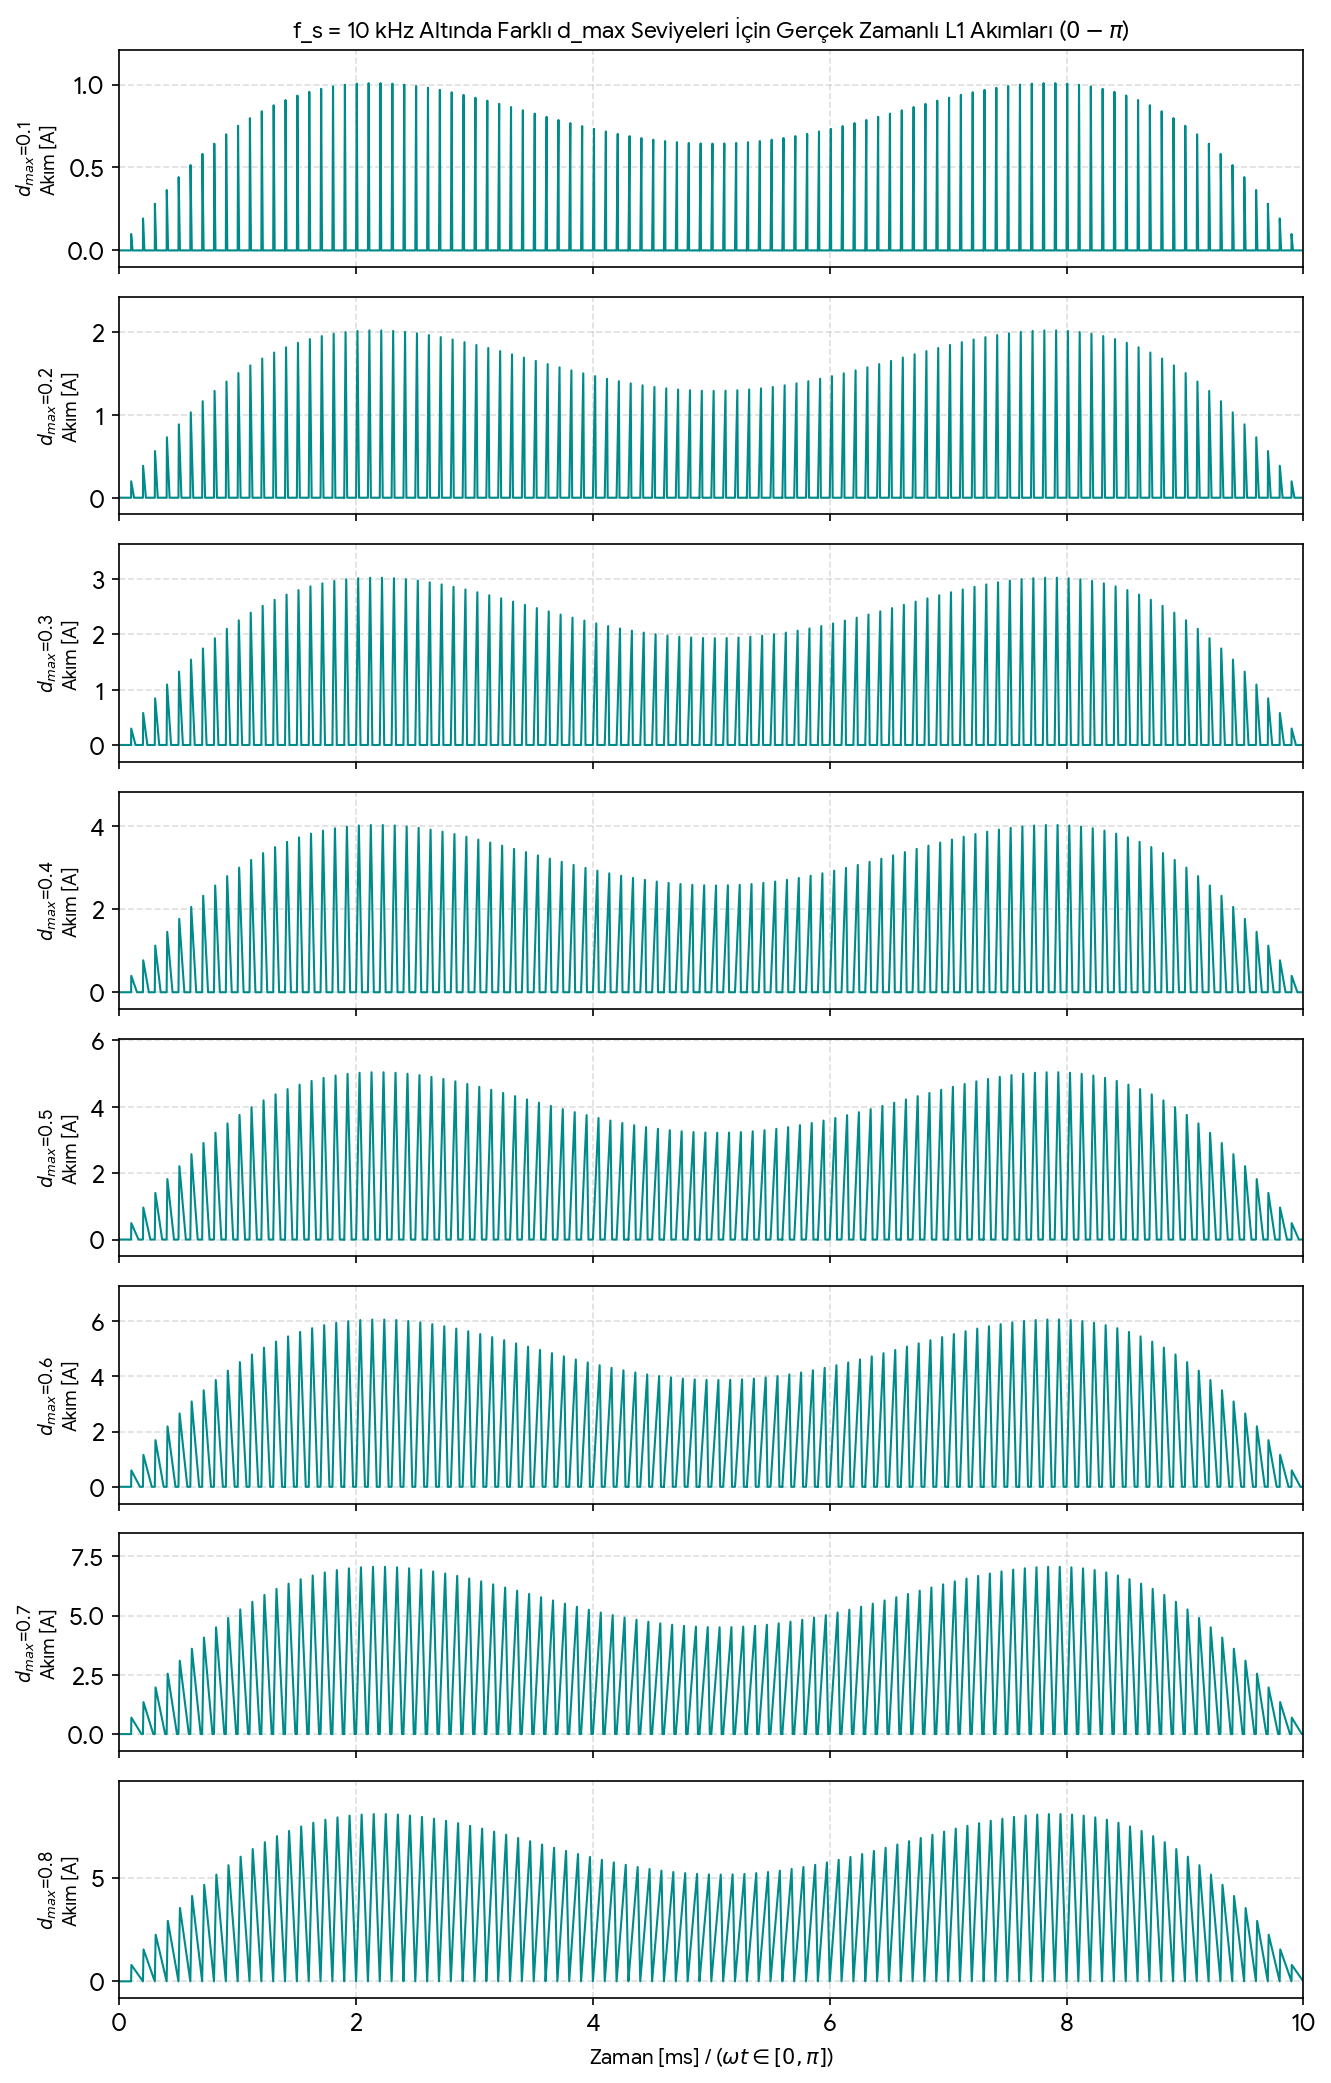
\includegraphics[width=0.76\textwidth]{sonuclar/eski_sekil_4_25_dcm_dmax.png}
  \caption{\eskitezetiketi\ Tam DCM varsayımı altında farklı $d_m$ değerleri için raporlanan $L_1$ akım darbeleri (eski Şekil 4.25; tarihsel analitik çıktı).}
  \label{fig:eski-dcm-dmax-taramasi}
\end{figure}

Eski sayısal katsayılar Tablo~\ref{tab:eski-dcm-harmonik-katsayilari} içinde birleştirilmiştir. Temel ve üçüncü harmonik genliklerinin $d_m^2$ ile birlikte ölçeklenmesi nedeniyle $I_3/I_1$ oranı bütün satırlarda yaklaşık \%43,93 kalmaktadır. Sabit oran yalnız tam DCM, ideal anahtar, seçilen gerilim modeli ve kip geçişi bulunmaması varsayımları altında elde edilen analitik sonuçtur; genel T-tipi evirici karakteristiği şeklinde yorumlanamaz.

\begin{table}[htbp]
  \centering
  \caption{\eskitezetiketi\ Eski tam-DCM modelinde raporlanan temel ve tek harmonik genlikleri ile üçüncü harmonik oranı.}
  \label{tab:eski-dcm-harmonik-katsayilari}
  \small
  \begin{tabular}{S[table-format=1.1] S[table-format=1.4] S[table-format=1.4] S[table-format=1.4] S[table-format=1.4] S[table-format=1.4] S[table-format=2.2]}
    \toprule
    {$d_m$} & {$I_1$ (A)} & {$I_3$ (A)} & {$I_5$ (A)} & {$I_7$ (A)} & {$I_9$ (A)} & {$100I_3/I_1$} \\
    \midrule
    0.1 & 0.0624 & 0.0274 & 0.0039 & 0.0013 & 0.0006 & 43.93 \\
    0.2 & 0.2497 & 0.1097 & 0.0157 & 0.0052 & 0.0024 & 43.93 \\
    0.3 & 0.5619 & 0.2468 & 0.0353 & 0.0118 & 0.0053 & 43.93 \\
    0.4 & 0.9989 & 0.4388 & 0.0627 & 0.0209 & 0.0095 & 43.93 \\
    0.5 & 1.5607 & 0.6856 & 0.0979 & 0.0326 & 0.0148 & 43.93 \\
    0.6 & 2.2475 & 0.9873 & 0.1410 & 0.0470 & 0.0214 & 43.93 \\
    0.7 & 3.0590 & 1.3438 & 0.1920 & 0.0640 & 0.0291 & 43.93 \\
    0.8 & 3.9955 & 1.7551 & 0.2507 & 0.0836 & 0.0380 & 43.93 \\
    \bottomrule
  \end{tabular}
\end{table}

\begin{figure}[H]
  \centering
  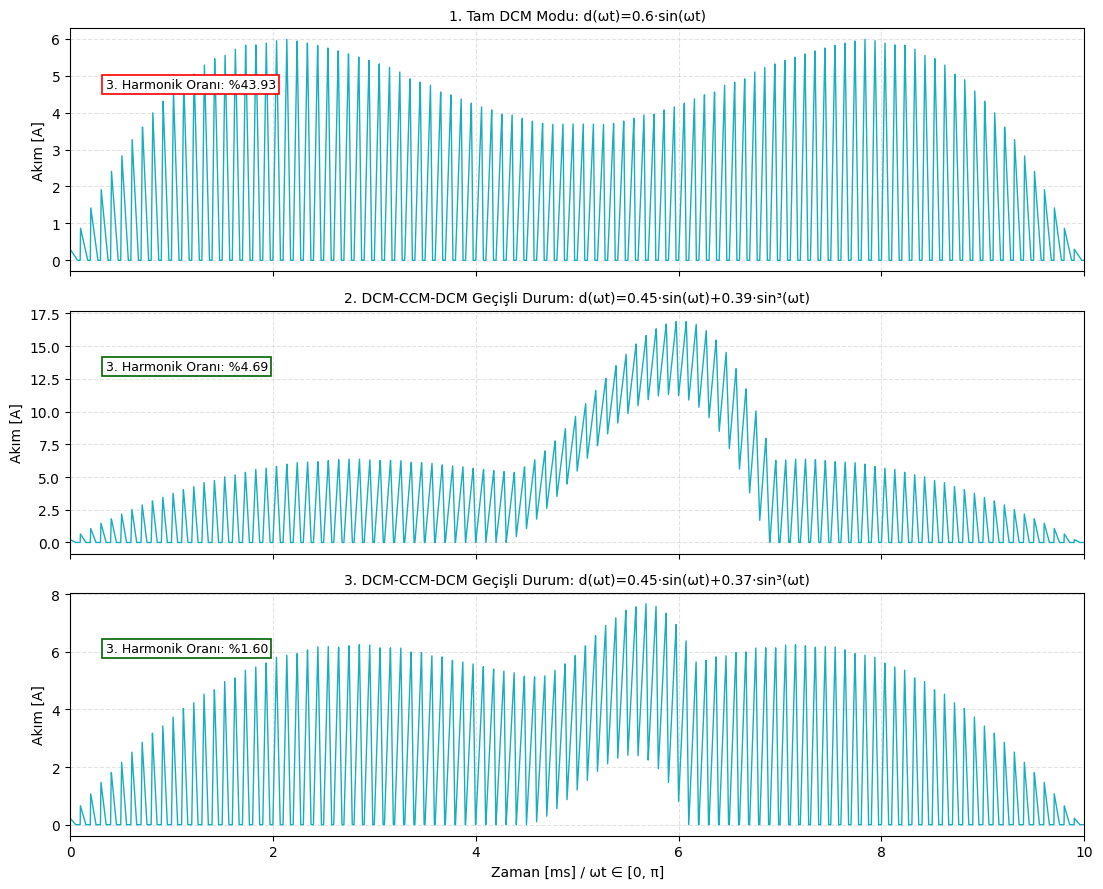
\includegraphics[width=0.82\textwidth]{sonuclar/eski_sekil_4_26_dcm_ccm.png}
  \caption{\eskitezetiketi\ Eski tezde tam DCM ile iki DCM--CCM--DCM adayının karşılaştırılması (eski Şekil 4.26; katsayı tanımı ve kip sınırları yeniden doğrulanacaktır).}
  \label{fig:eski-dcm-ccm-adaylari}
\end{figure}

Şekil~\ref{fig:eski-dcm-ccm-adaylari}, tam DCM durumundaki yüksek üçüncü harmonik oranını iki aday şekillendirme ile karşılaştırmaktadır. Şekil üzerindeki $d(\theta)=0{,}45\sin\theta+0{,}37\sin^3\theta$ gösterimi Eşitlik~\eqref{eq:sin3-esdeger-katsayilar} uyarınca hem temel hem üçüncü harmonik katsayısını değiştirir. Dolayısıyla eski metindeki $V_{1m}$ ve $V_{3m}$ adları doğrudan $\sin\theta$ ile $\sin(3\theta)$ katsayıları olarak okunmamalı; gerçek betik geldiğinde hangi parametrelemenin kullanıldığı belirlenmelidir.

\begin{figure}[H]
  \centering
  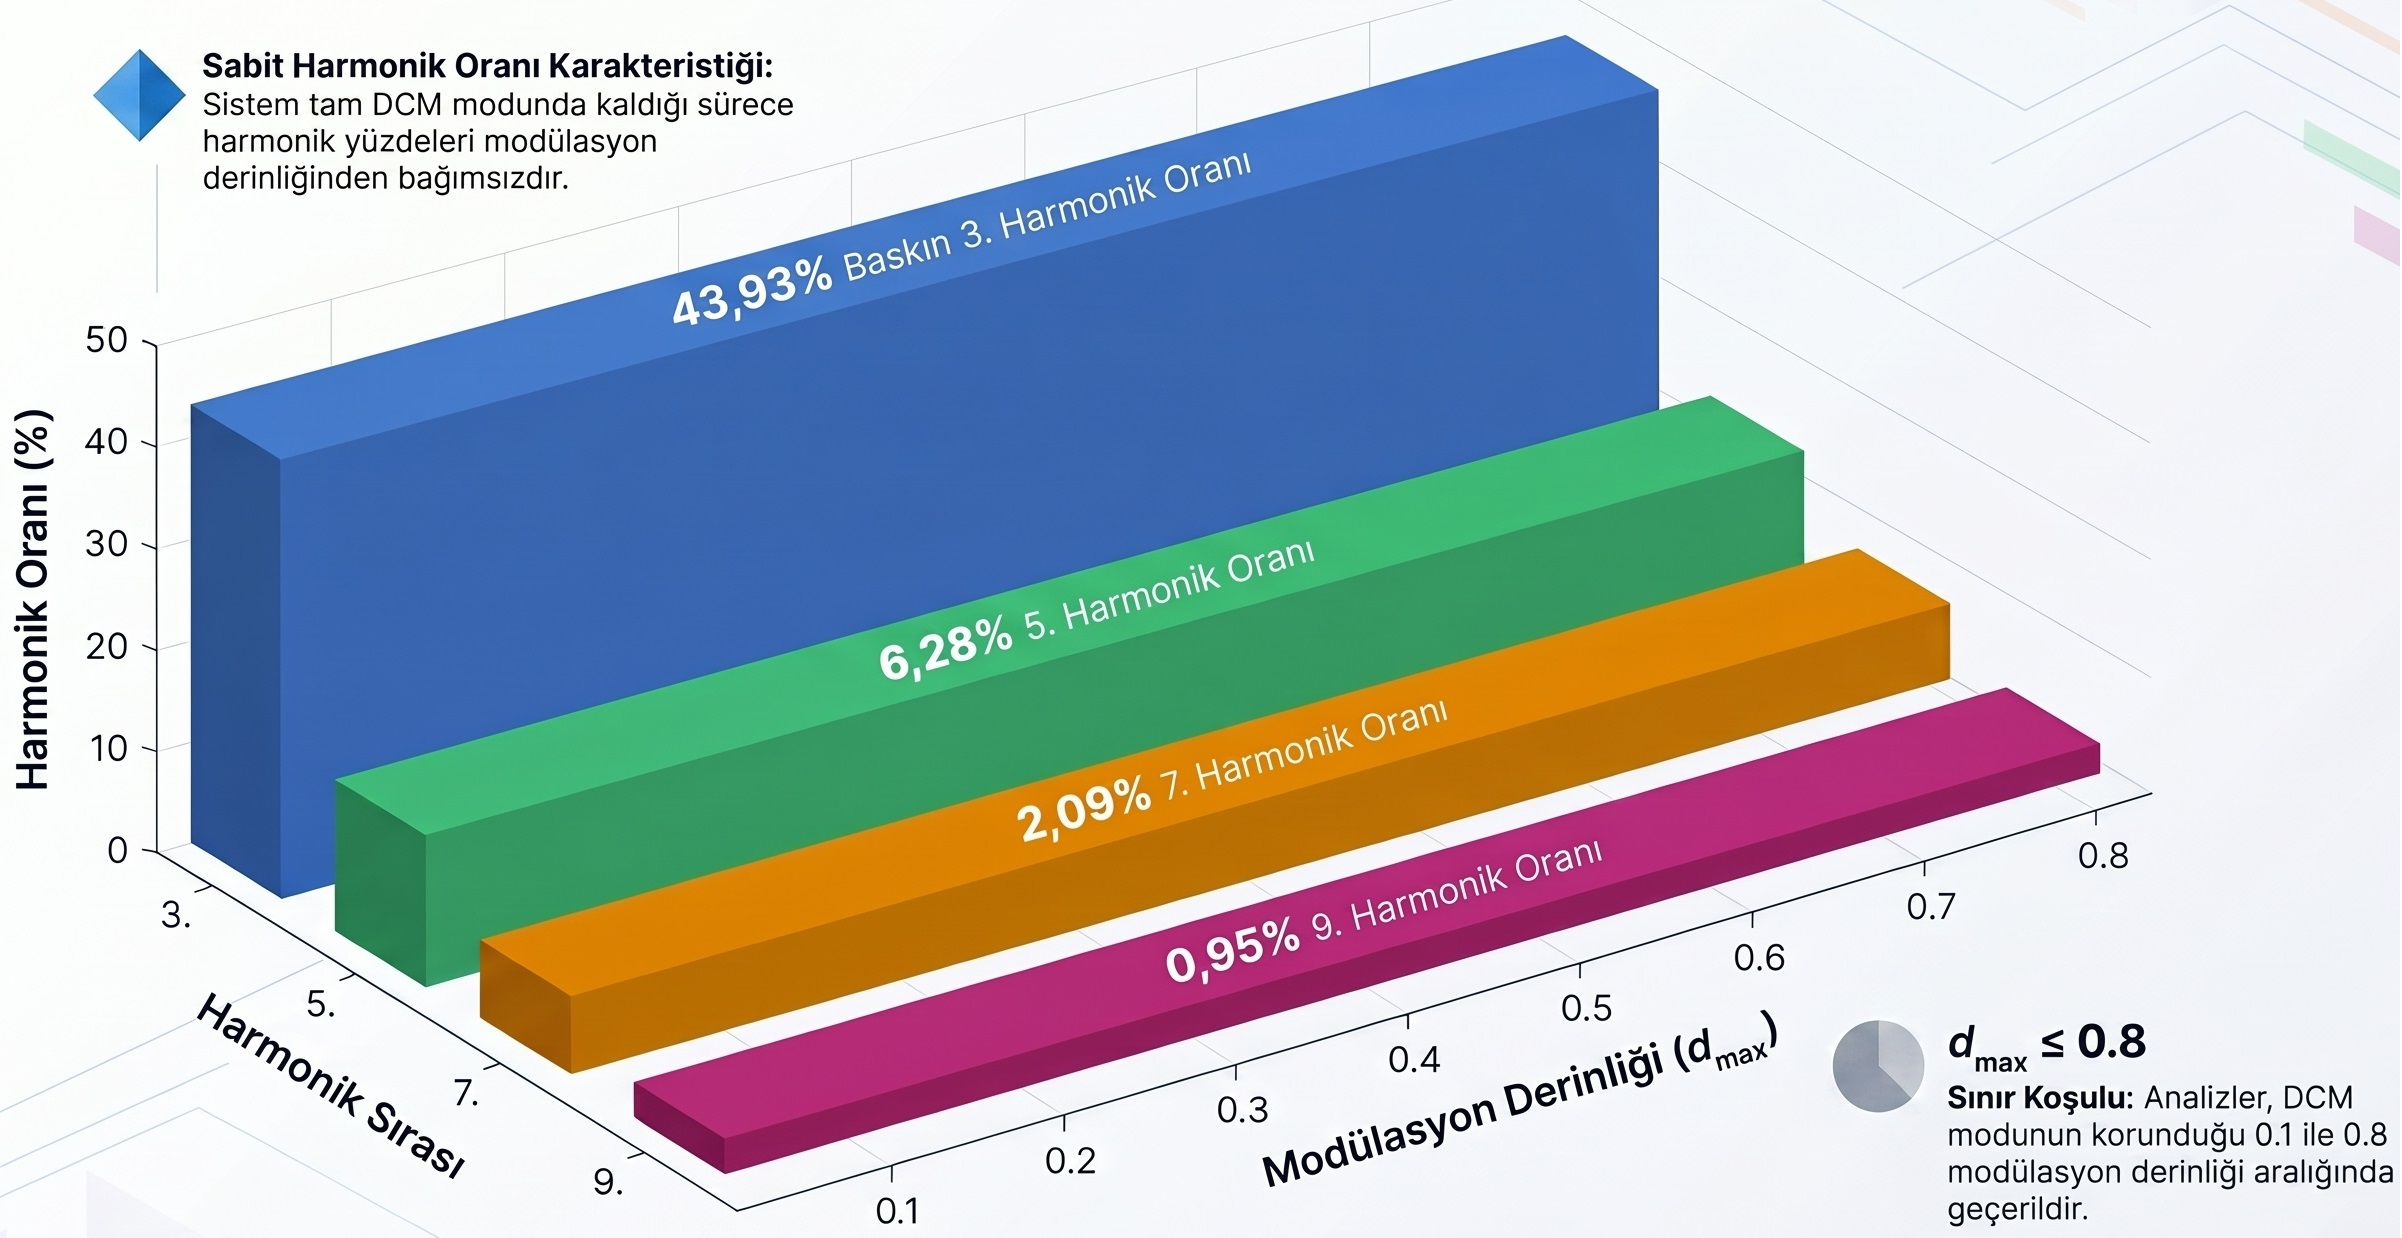
\includegraphics[width=0.87\textwidth]{sonuclar/eski_sekil_4_27_harmonik_dagilim.jpg}
  \caption{\eskitezetiketi\ Eski tam-DCM modelinde raporlanan sabit harmonik oranları (eski Şekil 4.27; yalnız belirtilen ideal model aralığı için geçerlidir).}
  \label{fig:eski-dcm-harmonik-dagilim}
\end{figure}

\begin{figure}[H]
  \centering
  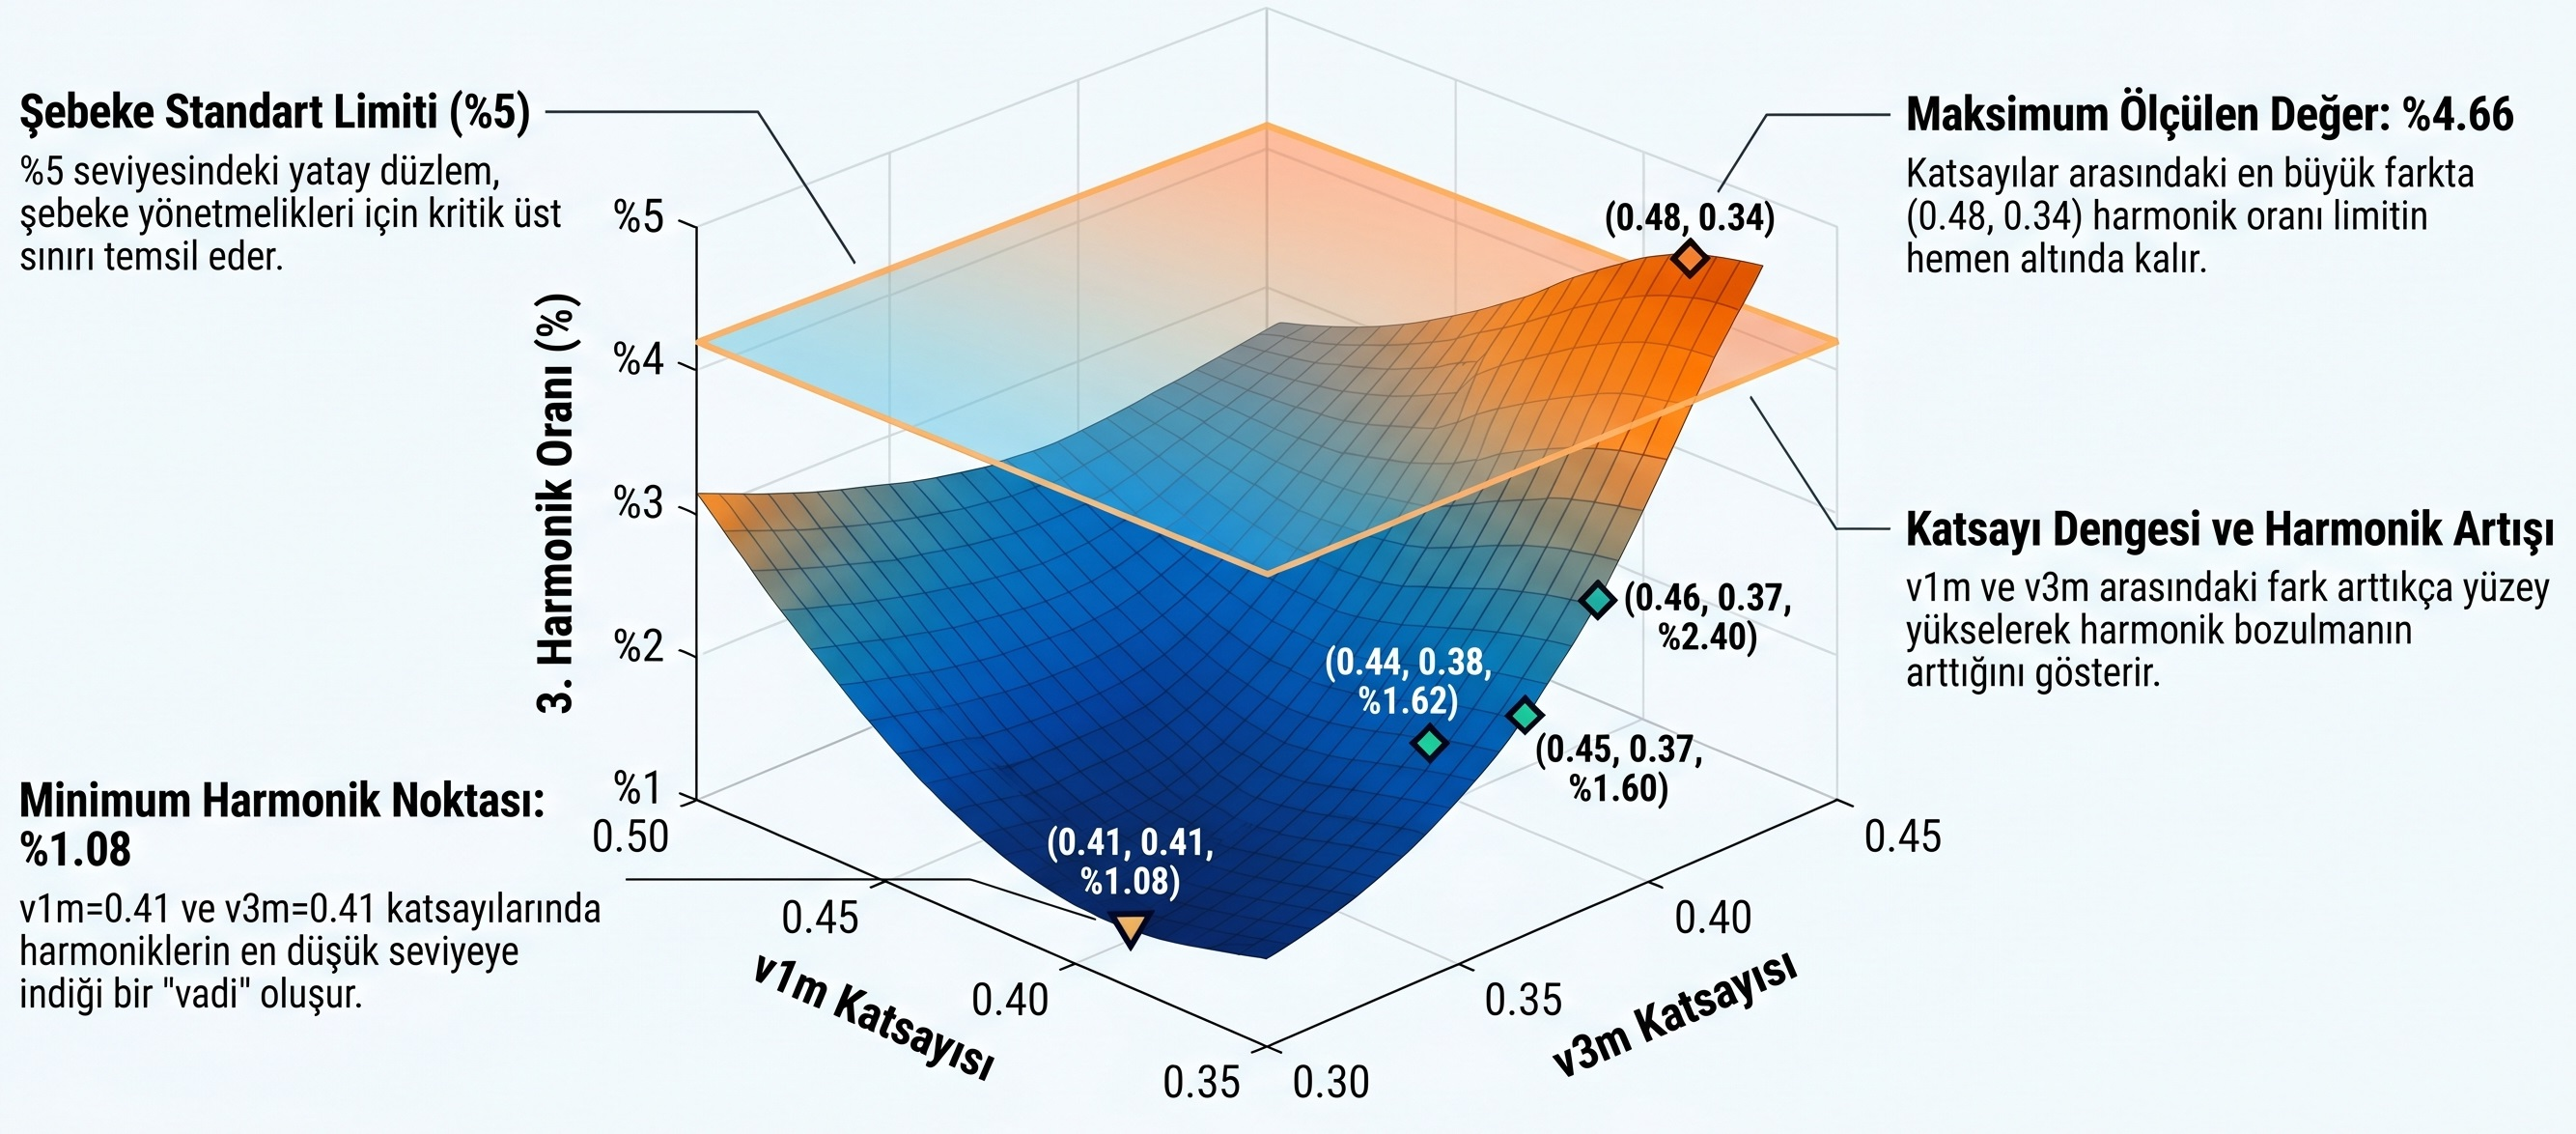
\includegraphics[width=0.94\textwidth]{sonuclar/eski_sekil_4_28_katsayi_yuzeyi.jpg}
  \caption{\eskitezetiketi\ Eski katsayı taramasından hazırlanan üçüncü harmonik yüzeyi (eski Şekil 4.28; tarihsel ve yeniden üretim bekleyen sonuç).}
  \label{fig:eski-katsayi-yuzeyi}
\end{figure}

\eskitezetiketi\ Eski Tablo~4.3, $I_{\mathrm{rms}}>\SI{2.2}{\ampere}$ ve $I_3/I_1<\%5$ koşullarını sağlayan 24 aday çift bildirmekte ve $(V_{1m},V_{3m})=(0{,}45,0{,}37)$ noktasında \%1,60 değerini öne çıkarmaktadır. Şekil~\ref{fig:eski-katsayi-yuzeyi} ise $(0{,}41,0{,}41)$ noktasında \%1,08 değerini minimum olarak göstermektedir. İki eski kayıt aynı optimumu vermediği için hiçbiri nihai katsayı seçimi sayılmamıştır. Katsayı yüzeyi, izin verilen modülasyon aralığı, RMS akım kısıtı, DCM--CCM geçiş koşulu ve Eşitlik~\eqref{eq:sin3-esdeger-katsayilar} ile tutarlı bir MATLAB betiği üzerinden yeniden hesaplanacaktır.

\tezcalismanotu{D5-2 --- Eski katsayı taraması ve Şekil 4.25--4.32'nin yeniden hesabı}{Eski Tablo~4.1--4.3 ile Şekil~4.25--4.32 tarihsel kanıt olarak korunmuş, çelişen optimum noktalar özellikle görünür bırakılmıştır. Gerçek yarım bara tanımı, $L_1/L_2/C_f$, anahtarlama frekansı, kip sınırı, akım referansı ve analiz penceresi kilitlendiğinde aday $K_1/K_3$ çiftleri aynı MATLAB betiğiyle yeniden taranacaktır. $I_3/I_1$, THD, RMS akım, ters akım alanı, modülasyon payı ve verim birlikte raporlanmadan hiçbir eski optimum nihai katsayı olarak seçilmeyecektir.}

\section{Önerilen Sin\texorpdfstring{\textsuperscript{3}}{3} Tabanlı İleri Besleme Yapısı ve Kontrol Blok Diyagramı}

Önceki tezin Şekil~4.17--4.21 dizisi klasik akım döngüsündeki şebeke gerilimi ileri beslemesini; Şekil~4.22 ve 4.23 ise doğrusal olmayan sistem yorumu ile önerilen kompanzasyon yolunu göstermektedir. Güncel işlevsel içerik Şekil~\ref{fig:denetim-modulasyon-blok} altında tek ve izlenebilir blok diyagramına dönüştürülmüştür. Akım hatası, $C_i(s)$ denetleyicisi, klasik $v_{\mathrm{ff}}$ yolu, Sin\textsuperscript{3} terimi, modülasyon sınırlayıcısı, PWM, nötr susturma mantığı ve T-tipi güç katı söz konusu diyagramda ayrı bloklar olarak korunmuştur. Görsel izlenebilirliği kaybetmemek amacıyla eski Şekil~4.18--4.22 de aşağıda özgün sıraları ve sarı tarihsel etiketleriyle ayrıca verilmiştir.

\eskitezetiketi\ Eski Şekil~4.18, evirici tarafındaki ileri besleme gerilim kaynağı ile şebeke eşdeğer kaynağının aynı genlik ve faza getirilmesi durumunu göstermektedir. İki kaynak arasındaki fark gerilimi sıfıra yaklaştığında seri $Z_1+Z_2$ empedansından akan akımın da sıfıra yaklaşması, ileri beslemenin akım başlamadan önceki senkron eşpotansiyel durumunu açıklamaktadır.

\begin{figure}[htbp]
  \centering
  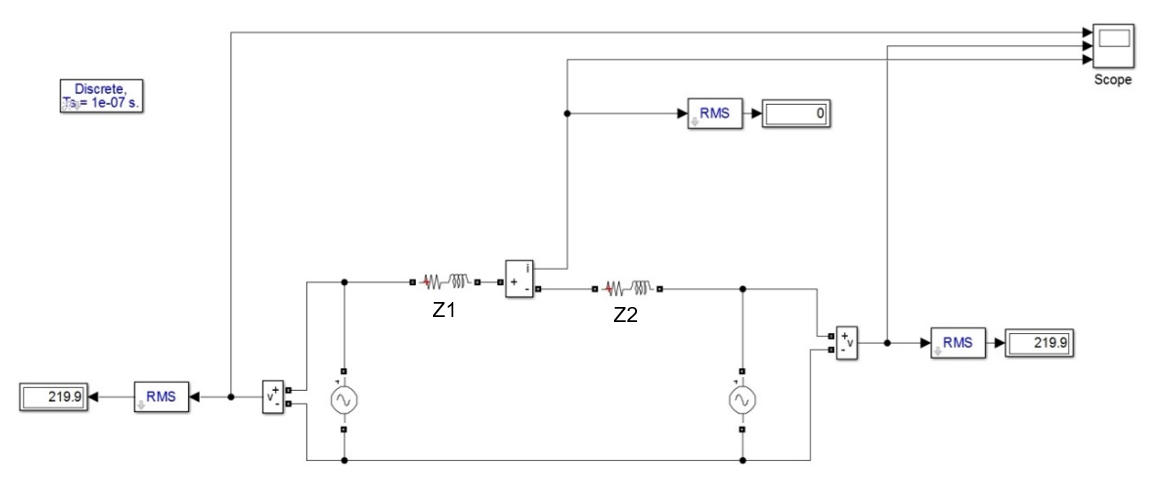
\includegraphics[width=0.96\textwidth]{sonuclar/eski_sekil_4_18_feedforward_etkisi.png}
  \caption{\eskitezetiketi\ İleri besleme bileşeninin eşdeğer kaynaklar ve seri empedanslar üzerindeki etkisini gösteren tarihsel benzetim modeli (eski Şekil 4.18).}
  \label{fig:eski-feedforward-etkisi}
\end{figure}

Şekil~\ref{fig:eski-espotansiyel-dalga}, Şekil~\ref{fig:eski-feedforward-etkisi} altında tanımlanan iki eşpotansiyel kaynağın gerilim dalga biçimlerini ve kaynaklar arasındaki akımın sıfır oluşunu birlikte göstermektedir. Kayıt, PLL ile şebekeye senkron olunduktan sonra aktif akım komutu uygulanmadan önce beklenen başlangıç durumunun görsel karşılığıdır; kapalı çevrim izleme performansını tek başına kanıtlamamaktadır.

\begin{figure}[htbp]
  \centering
  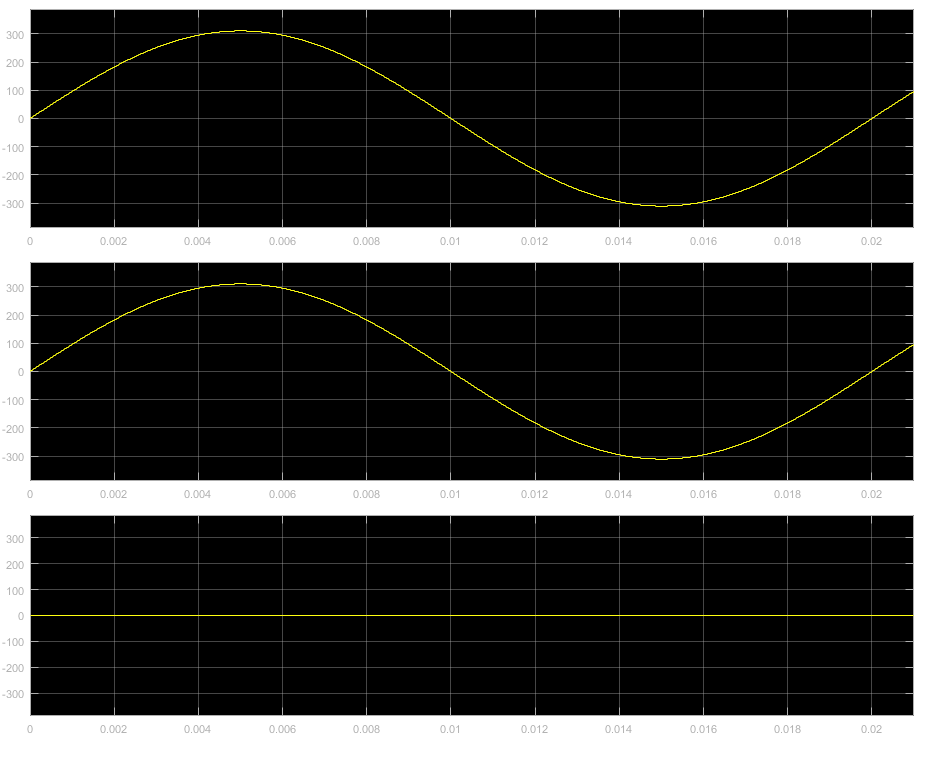
\includegraphics[width=0.90\textwidth]{sonuclar/eski_sekil_4_19_espotansiyel_dalga.png}
  \caption{\eskitezetiketi\ Eşpotansiyel kaynakların gerilim dalga biçimleri ve kaynaklar arasındaki akımın sıfır oluşu (eski Şekil 4.19).}
  \label{fig:eski-espotansiyel-dalga}
\end{figure}

\eskitezetiketi\ Eski anlatımda akımın yükselmesi için denetleyici çıkışının, klasik ileri besleme gerilimine filtre ve şebeke empedanslarındaki düşümü karşılayacak bir gerilim eklediği kabul edilmiştir. Şekil~\ref{fig:eski-tam-guc-feedforward}, tam güç olarak adlandırılan çalışma noktasında ileri besleme, denetleyici ve ana kaynak katkılarını; Şekil~\ref{fig:eski-dusuk-guc-feedforward} ise aynı ayrımı yaklaşık \SI{2.7}{\ampere} faz akımında göstermektedir. İki kayıt, akım azaldıkça denetleyici tarafından üretilmesi gereken mutlak ek gerilimin küçüldüğünü ve küçük gerilim/model hatalarının düşük akımda göreli olarak daha görünür hâle geldiğini açıklamak için korunmuştur.

\begin{figure}[htbp]
  \centering
  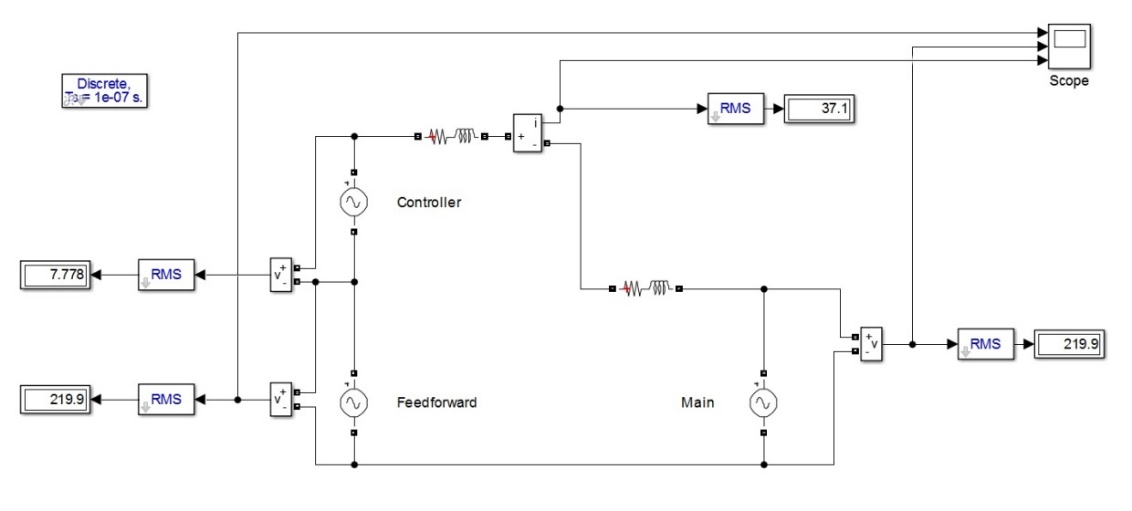
\includegraphics[width=0.94\textwidth]{sonuclar/eski_sekil_4_20_tam_guc_feedforward.jpg}
  \caption{\eskitezetiketi\ Evirici tam güçte iken ileri besleme ve denetleyici gerilim katkılarının tarihsel eşdeğer devre üzerinde gösterimi (eski Şekil 4.20).}
  \label{fig:eski-tam-guc-feedforward}
\end{figure}

\begin{figure}[htbp]
  \centering
  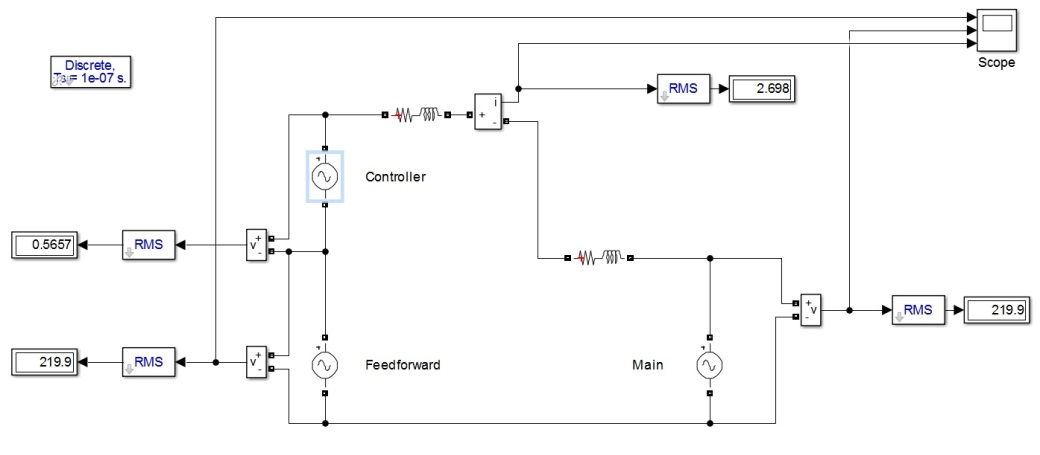
\includegraphics[width=0.94\textwidth]{sonuclar/eski_sekil_4_21_dusuk_guc_feedforward.jpg}
  \caption{\eskitezetiketi\ Yaklaşık \SI{2.7}{\ampere} faz akımında ileri besleme ve denetleyici gerilim katkılarının tarihsel eşdeğer devre üzerinde gösterimi (eski Şekil 4.21).}
  \label{fig:eski-dusuk-guc-feedforward}
\end{figure}

Eski tezin verdiği $L_1=\SI{650}{\micro\henry}$, $C_f=\SI{8}{\micro\farad}$ ve $L_2=\SI{150}{\micro\henry}$ değerleri yalnız tarihsel model parametreleridir. İdeal seri eşdeğer yaklaşımda \SI{50}{\hertz} çevresindeki $\SI{0.25132}{\ohm}$ reaktans değeri kullanılırsa \SI{37.1}{\ampere} için gerilim düşümü yaklaşık \SI{9.32}{\volt}, \SI{2.7}{\ampere} için ise yaklaşık \SI{0.68}{\volt} olur. Eski Şekil~4.20 üzerindeki \SI{7.778}{\volt} ve eski Şekil~4.21 üzerindeki \SI{0.5657}{\volt} denetleyici çıkışları, aynı bölümün metninde sırasıyla \SI{9.324}{\volt} ve \SI{0.578}{\volt} olarak açıklanmıştır. Görsel, metin ve ideal çarpım aynı sayısal sonucu vermediğinden değerler nihai model doğrulaması olarak kullanılmamıştır. Ayrım, ileri besleme teriminin düşük akımda göreli öneminin arttığı yönündeki fiziksel yorumu ortadan kaldırmamakta; gerçek modelde empedansın, RMS tanımının ve ölçüm noktalarının birlikte doğrulanmasını gerektirmektedir.

Şekil~\ref{fig:eski-dogrusal-olmayan-sistem}, eski tezde anahtarlama bloğu ile $L_1$--$C_f$--$L_2$ filtresinin birlikte $G(s)$ adı altında gösterildiği fiziksel sınırı korumaktadır. Şema tek başına doğrusal olmama durumunu kanıtlamaz; çalışma noktasına bağlı anahtarlama, DCM--CCM kip geçişi, doyum ve periyodik katsayılar doğrusal olmayan veya doğrusal zamanla periyodik davranışın asıl kaynaklarıdır. Eşitlik~\eqref{eq:dcm-ortalama-akim}--\eqref{eq:dcm-kritik-gorev} ilgili tarihsel yorumun güncel matematiksel karşılığını vermektedir.

\begin{figure}[htbp]
  \centering
  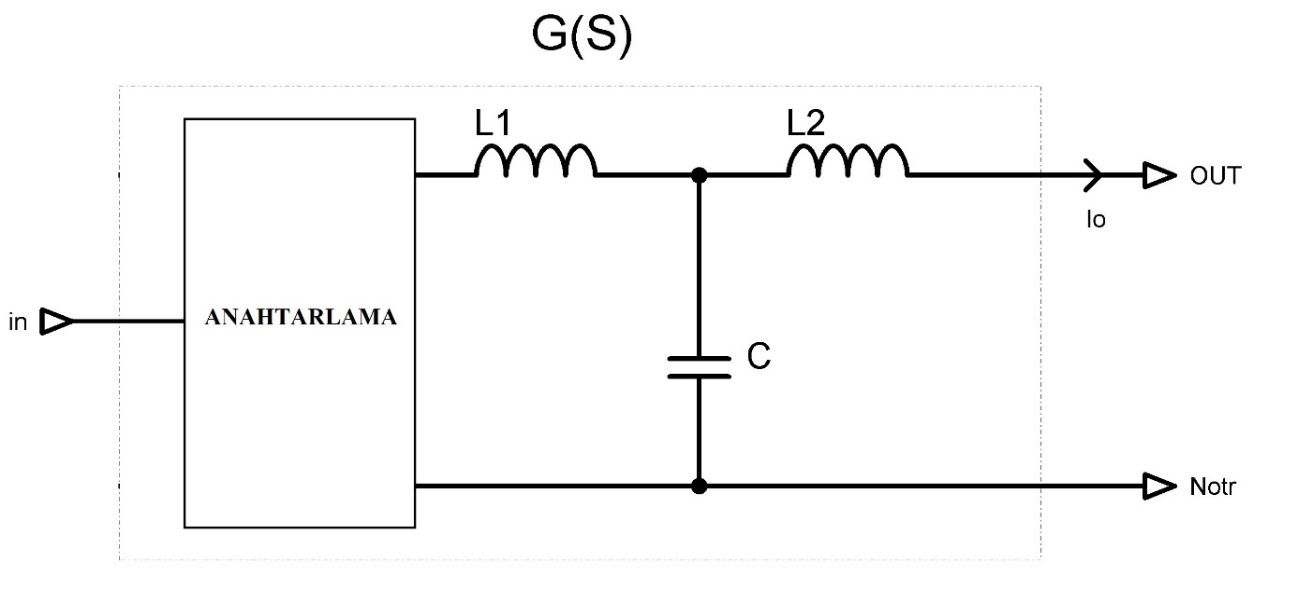
\includegraphics[width=0.92\textwidth]{sonuclar/eski_sekil_4_22_dogrusal_olmayan_sistem.jpg}
  \caption{\eskitezetiketi\ Anahtarlama katı ile $L_1$--$C_f$--$L_2$ çıkış filtresinin tarihsel sistem sınırı gösterimi (eski Şekil 4.22).}
  \label{fig:eski-dogrusal-olmayan-sistem}
\end{figure}

\eskitezetiketi\ Eski anlatımda denetleyici devre dışı bırakılarak yalnız ileri besleme katsayısının değiştirildiği benzetim koşulu, yöntemin açık çevrim mekanizmasını ayırmak için yararlı bir deneydir. Aynı koşul kapalı çevrim performansı veya kararlılık kanıtı değildir. Şebeke gerilimi ileri beslemesi ideal durumda evirici ile şebeke gerilimini yaklaştırarak düşük akımdaki göreli gerilim hatasını azaltabilir; LCL filtre, PCC ölçümü ve dijital gecikme eklendiğinde aynı yol sanal empedans ve aktif sönümleme etkisi de oluşturabilir \citep{Lu2016}. İleri besleme yolunun etkisi bu nedenle yalnız gerilim düşümü hesabıyla sınırlandırılmamıştır.

\tezcalismanotu{D5-3 --- Eski Şekil 4.17--4.23'ün blok düzeyinde bire bir denetimi}{Eski kontrol ve ileri besleme şekilleri yeni işlevsel blok diyagramında birleştirilmiş, eski Şekil~4.18--4.22 ayrıca tarihsel izlenebilirlik için tutulmuştur. Kesin kontrol kodu geldiğinde PCC/şebeke geriliminin alındığı nokta, ölçekleme, denetleyicinin açık/kapalı durumu, toplama işaretleri, sınırlayıcı sırası, gecikmeler ve PWM kazancı eski şekillerle satır satır karşılaştırılacaktır. Farklı bir bağlantı veya sıra görülürse güncel blok diyagramı ve çevre metin birlikte düzeltilecektir.}

\section{Kapalı Çevrim Modeli}

Faz başına gerilimden akıma LCL bitkisi $G_{vi}(s)$ Bölüm~\ref{chap:sistem} içinde Eşitlik~\eqref{eq:lcl-aktarim} ile tanımlanmıştır. PR denetleyicisi $C_i(s)$ Eşitlik~\eqref{eq:pr-denetleyici}, normalize modülasyon komutunu evirici kutup gerilimine dönüştüren PWM eşdeğer kazancı $K_{\mathrm{pwm}}$ ve toplam hesaplama--örnekleme--PWM gecikmesi $G_d(s)$ ile gösterilsin. Boyutsuz açık çevrim kazanç fonksiyonu $L(s)$
\begin{equation}
  L(s)=C_i(s)K_{\mathrm{pwm}}G_d(s)G_{vi}(s)
  \label{eq:sin3-acik-cevrim}
\end{equation}
olarak yazılır. Eşitlik~\eqref{eq:sin3-acik-cevrim} içindeki çarpanlar aynı işaret yönü ve birim sistemiyle kurulmalıdır. Toplam gecikme süresi $T_d$ olmak üzere sürekli-zaman yaklaşımında $G_d(s)=\exp(-sT_d)$ kullanılabilir; rasyonel Bode hesabında ise mertebesi belirtilmiş Padé yaklaşımı uygulanır. PR yapısının temel frekansta yüksek kazanç sağlaması sinüzoidal izleme hatasını azaltırken LCL rezonansı ek sönümleme veya uygun aktif sönümleme tasarımı gerektirir \citep{Teodorescu2006PR,Zhang2014PR}.

Referans izleme ve bozucu bastırma incelemesinde duyarlılık fonksiyonları
\begin{equation}
  S(s)=\frac{1}{1+L(s)},
  \qquad
  T(s)=\frac{L(s)}{1+L(s)}
  \label{eq:sin3-duyarlilik}
\end{equation}
biçimindedir. Eşitlik~\eqref{eq:sin3-duyarlilik} içindeki $S(s)$ duyarlılık, $T(s)$ tamamlayıcı duyarlılık fonksiyonudur. Doğrusal modelde toplama noktasına dışsal olarak eklenen $u_{\mathrm{ff},\sin^3}$ terimi Eşitlik~\eqref{eq:sin3-acik-cevrim} içindeki karakteristik paydayı tek başına değiştirmez. Buna karşılık gerçek uygulamada doygunluk, örnekleme, PLL faz hatası, anahtarlama kip değişimi ve PCC gerilimi üzerinden oluşan iç bağlaşım söz konusu ayrımı bozabilir. Şebeke gerilimi ileri beslemesinin dijital gecikmeyle birlikte LCL rezonansına sönümleme veya kararsızlaştırıcı etki verebilmesi literatürde hem model hem deneyle gösterilmiştir \citep{Lu2016,Wang2024}.

Şebeke akımı, akım referansı, Sin\textsuperscript{3} ileri besleme komutu ve şebeke geriliminin Laplace dönüşümleri sırasıyla $I_g(s)$, $I^{\ast}(s)$, $U_{\mathrm{ff},\sin^3}(s)$ ve $V_g(s)$ ile; şebeke geriliminden akıma bozucu aktarım $G_{vg}(s)$ ile gösterilsin. Harmonik kompanzasyonun doğrusal küçük işaret modeli, seçilen çalışma noktası çevresinde
\begin{equation}
  I_g(s)=T(s)I^{\ast}(s)+S(s)K_{\mathrm{pwm}}G_d(s)G_{vi}(s)U_{\mathrm{ff},\sin^3}(s)
  +S(s)G_{vg}(s)V_g(s)
  \label{eq:sin3-kapali-cevrim-girisleri}
\end{equation}
şeklinde ayrıştırılabilir. $G_{vg}(s)$'nin işareti seçilen gerilim ve akım yönlerine bağlıdır. Eşitlik~\eqref{eq:sin3-kapali-cevrim-girisleri}, Sin\textsuperscript{3} yolunun akım geri beslemesiyle seri bir denetleyici olmadığını; kapalı çevrim tarafından süzülen ayrı bir giriş olduğunu göstermektedir.

\tezcalismanotu{D5-4 --- Kapalı çevrim ve HTF doğrulaması}{Geçici Bode çıktısı yöntem akışını göstermektedir; sayısal kazanç/faz marjı sonucu değildir. Gerçek LCL, PR, örnekleme, hesaplama ve PWM gecikmeleri geldiğinde $L(s)$, $S(s)$ ve $T(s)$ yeniden üretilecek; düşük, orta ve nominal güçte çalışma noktası duyarlılığı denetlenecektir. Nötr susturma nedeniyle harmonikler arası bağlaşım anlamlıysa temel--üçüncü harmonik HTF matrisi model doğrusallaştırması veya küçük işaret enjeksiyonuyla çıkarılacak ve kesme mertebesi/hata ölçütü raporlanacaktır.}

\section{Bode ve Kararlılık Marjı Analizi}

\juriistegietiketi\ Jüri talebi doğrultusunda $L(s)$, $S(s)$ ve $T(s)$ aynı fiziksel bitki, denetleyici ve gecikme modeliyle birlikte incelenmiştir. Gerçek $L_1$, $L_2$, $C_f$, sönümleme, PR katsayıları, örnekleme süresi ve gecikme henüz kilitlenmediğinden Şekil~\ref{fig:gecici-bode-lst} nihai kararlılık kanıtı değil, analiz zincirinin çalışan MATLAB çıktısıdır. Geçici parametrelerle elde edilen eğrilerin tezde tutulması yöntemi görünür kılmakta; sayısal marjların gerçek kod ve model geldiğinde aynı betikle değiştirilmesini sağlamaktadır.

\begin{figure}[htbp]
  \centering
  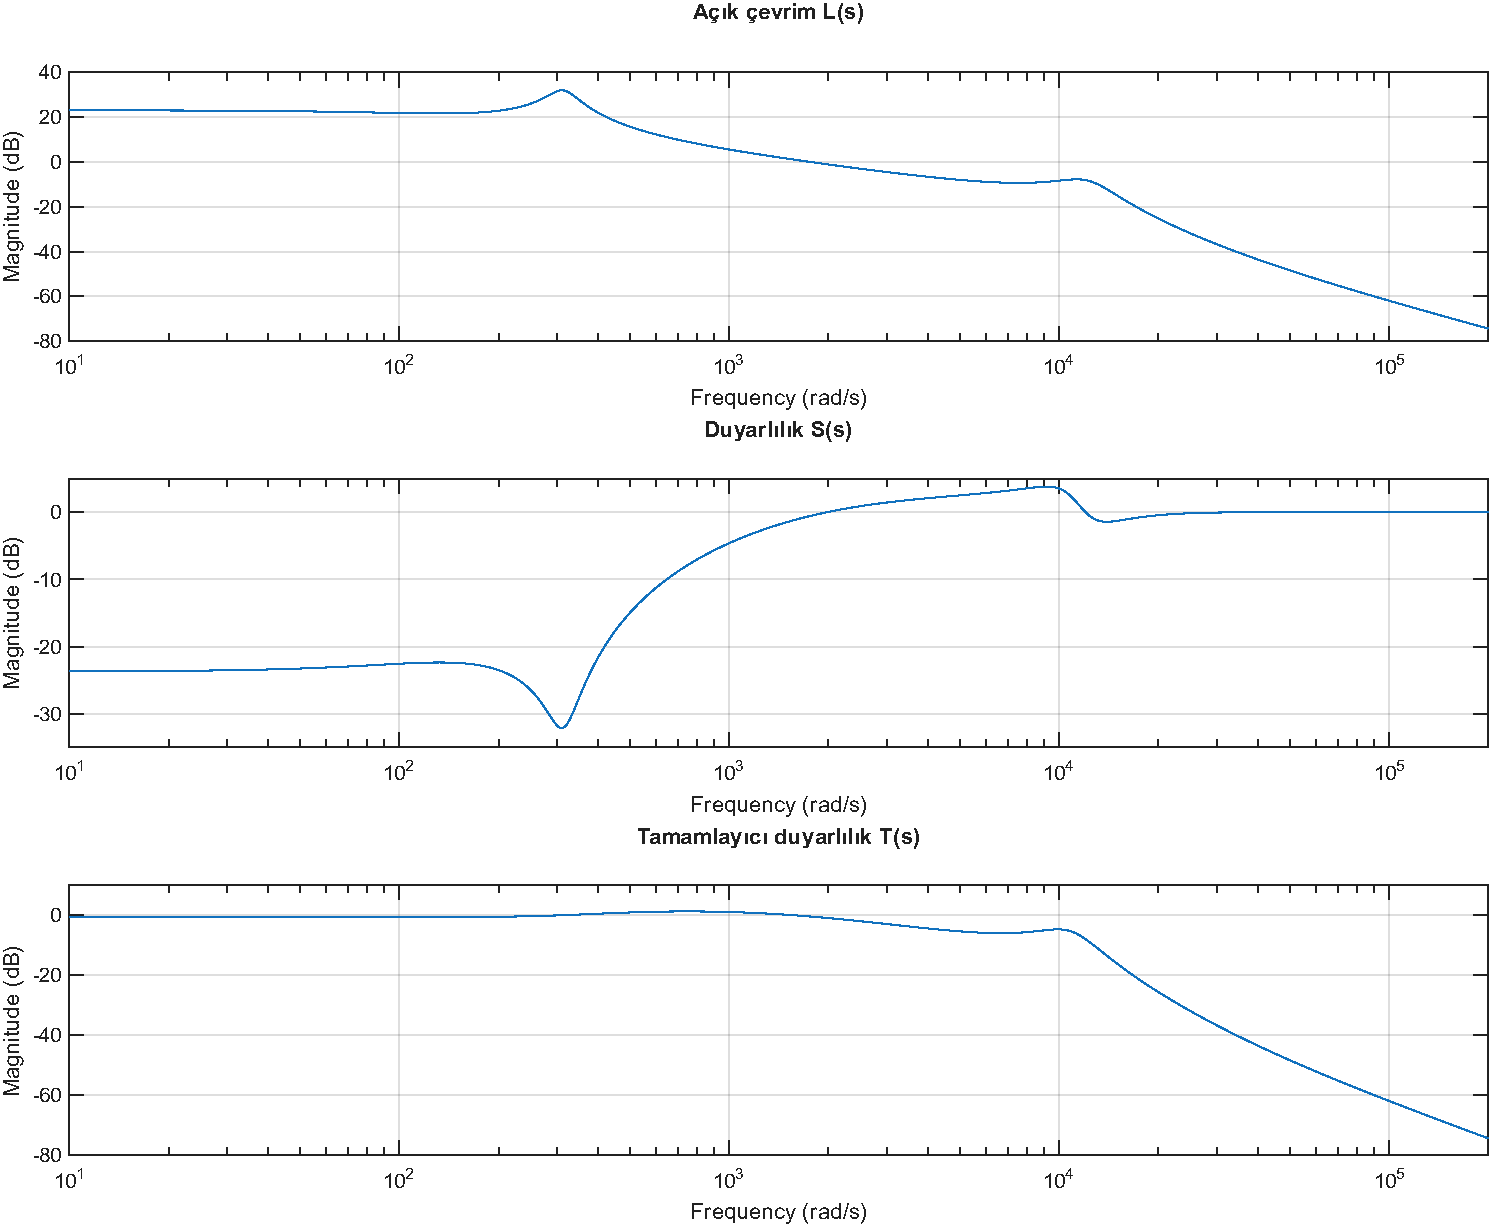
\includegraphics[width=0.96\textwidth]{../tez-matlab-simulink/results/stability/bode_LST.pdf}
  \caption{\juriistegietiketi\ Geçici LCL--PR--gecikme modeli için MATLAB ile üretilen $L(s)$, $S(s)$ ve $T(s)$ büyüklük eğrileri; nihai parametre doğrulaması beklenmektedir.}
  \label{fig:gecici-bode-lst}
\end{figure}

Geçici modelde toplam gecikme \SI{150}{\micro\second} alınmış, kazanç marjı \SI{9.09}{\decibel} ve faz marjı $64{,}16^{\circ}$ hesaplanmıştır. Ek şebeke endüktansı $0$--\SI{2}{\milli\henry} arasında tarandığında aday model kararlı kalmış ve faz marjı $61{,}40^{\circ}$--$64{,}16^{\circ}$ aralığında değişmiştir. Sonuçlar yalnız analiz betiğinin çalıştığını göstermektedir; gerçek denetleyici katsayıları ve gecikme doğrulanmadan tezin nihai kararlılık marjı olarak savunulmayacaktır.

\begin{table}[htbp]
  \centering
  \caption{\juriistegietiketi\ Kapalı çevrim kararlılık incelemesinin tamamlanma ölçütleri.}
  \label{tab:sin3-kararlilik-kontrol-listesi}
  \small
  \begin{tabularx}{\textwidth}{p{0.24\textwidth} X p{0.24\textwidth}}
    \toprule
    İnceleme & Değişkenler ve raporlanacak çıktı & Mevcut durum \\
    \midrule
    Nominal model & $L,S,T$, kesişim frekansları, kazanç/faz marjı & Geçici MATLAB çıktısı mevcut \\
    Şebeke dayanıklılığı & $R_g,L_g$ taraması ve en kötü marj & $L_g=0$--\SI{2}{\milli\henry} geçici taraması mevcut \\
    Sayısal gecikme & Örnekleme, hesaplama, PWM güncelleme ve ölçüm filtresi & Gerçek kodla doğrulanacak \\
    Çalışma noktası & Düşük, orta ve anma gücünde kip/doğrusallaştırma geçerliliği & Gerçek modelle doğrulanacak \\
    Doğrusal olmayan sınırlar & Modülasyon doyumu, akım sınırlama, nötr susturma geçişi & Zaman alanı testiyle doğrulanacak \\
    \bottomrule
  \end{tabularx}
\end{table}

Klasik LTI Bode incelemesi seçilen çalışma noktası çevresindeki yerel dinamiği verir. Nötr susturma periyodik kip değiştirdiği için harmonikler arası bağlaşım önemli hâle gelirse HTF veya harmonik durum uzayı modeli ayrıca kurulmalıdır. HTF'nin sonsuz mertebeli matris yapısı, sonlu model için kesme mertebesi ve hata ölçütü gerektirir \citep{Liao2022}. Ham frekans taraması gelmeden skaler bir ``üçüncü harmonik transfer fonksiyonu'' üzerinden kararlılık iddiası kurulmamıştır.

\section{Düşük, Orta ve Nominal Güç Karşılaştırması}

Kurtarılan Senaryo~3 ekranları, Sin\textsuperscript{3} kompanzasyonunun eski tezdeki görsel kanıt zincirini tamamlamaktadır. Şekil~\ref{fig:sin3-l1-yakin}, kompanzasyonlu $L_1$ akımının anahtarlama ölçeğindeki yapısını; Şekil~\ref{fig:sin3-dort-kanal} gerilim ve akım kanallarını ortak zaman ekseninde; Şekil~\ref{fig:sin3-l1-fft} ile Şekil~\ref{fig:sin3-iout-fft} ise iki akım ölçüm noktasındaki harmonik sonuçları göstermektedir.

\begin{figure}[H]
  \centering
  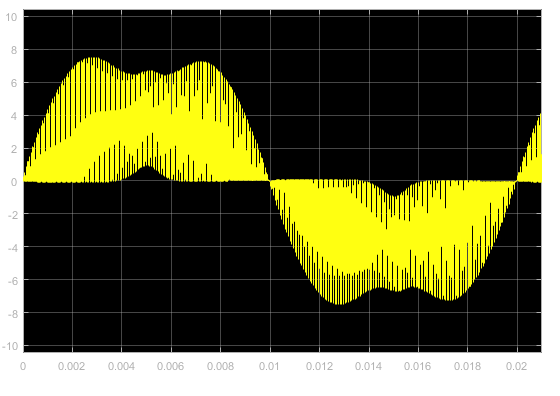
\includegraphics[width=0.82\textwidth]{sonuclar/eski_sekil_4_29_sin3_l1.png}
  \caption{\eskitezetiketi\ Sin\textsuperscript{3} kompanzasyonlu nötr susturma benzetiminde $L_1$ akımının büyütülmüş görünümü (eski Şekil 4.29).}
  \label{fig:sin3-l1-yakin}
\end{figure}

\begin{figure}[H]
  \centering
  \includegraphics[width=0.98\textwidth]{../dosyalar/05_sonradan_gelenler/Senaryo_3/dalga_sekilleri_s3.jpg}
  \caption{\eskitezetiketi\ Sin\textsuperscript{3} kompanzasyonlu yöntemde filtre girişi gerilimi, filtrelenmiş gerilim, $L_1$ akımı ve çıkış akımı (eski Şekil 4.30'un yüksek çözünürlüklü kaydı).}
  \label{fig:sin3-dort-kanal}
\end{figure}

Şekil~\ref{fig:sin3-dort-kanal} altındaki ilk kanal T-tipi anahtarlama gerilimini, ikinci kanal filtrelenmiş gerilimi, üçüncü kanal $L_1$ endüktör akımını ve dördüncü kanal LC filtre çıkış akımını göstermektedir. Susturma yönteminin Şekil~\ref{fig:susturma-dort-kanal} altındaki belirgin zarf bozulması kompanzasyon sonrasında azalmış; ancak çıkış akımı klasik yöntemdeki kadar sinüzoidal hâle gelmemiştir. Görsel karşılaştırma, aynı analiz penceresindeki FFT değerleriyle birlikte okunmalıdır.

\begin{figure}[H]
  \centering
  \includegraphics[width=0.98\textwidth]{../dosyalar/05_sonradan_gelenler/Senaryo_3/THD_IL1.jpg}
  \caption{\eskitezetiketi\ Sin\textsuperscript{3} kompanzasyonlu yöntemde $L_1$ akımı FFT sonucu: temel bileşen \SI{3.752}{\ampere}, $\mathrm{THD}_{L1}=\%9{,}46$ (eski Şekil 4.31).}
  \label{fig:sin3-l1-fft}
\end{figure}

\begin{figure}[H]
  \centering
  \includegraphics[width=0.98\textwidth]{../dosyalar/05_sonradan_gelenler/Senaryo_3/THD_Iout.jpg}
  \caption{\eskitezetiketi\ Sin\textsuperscript{3} kompanzasyonlu yöntemde çıkış akımı FFT sonucu: temel bileşen \SI{3.766}{\ampere}, $\mathrm{THD}_{\mathrm{out}}=\%7{,}79$ (eski Şekil 4.32).}
  \label{fig:sin3-iout-fft}
\end{figure}

Senaryo~3'te $L_1$ THD değeri susturma durumundaki \%46,86'dan \%9,46'ya, çıkış THD değeri ise \%46,35'ten \%7,79'a düşmüştür. İyileşme, Sin\textsuperscript{3} yolunun eski modelde üçüncü harmonik cezasını önemli ölçüde azalttığını desteklemektedir. Klasik çıkış THD değerinin \%2,14 olması, kompanzasyonlu yöntemin harmonik bakımından klasik yöntemi geçmediğini de açıkça gösterir. Eski tezde verilen \%93,70 verim değeri ham kayıp modeli bulunmadığından yeniden doğrulanmış bir sonuç değildir.

\juriistegietiketi\ Düşük, orta ve nominal güçte aynı denetim yapısının karşılaştırılması henüz tamamlanmış bir sonuç tablosu değildir. Mevcut arşiv yalnız düşük güç ekranlarını sağlamaktadır. Geçici MATLAB güç taraması yöntem geliştirme amacıyla yapılmış olsa da gerçek anma gücü, filtre, denetleyici ve anahtarlama mantığı doğrulanmadığından tez bulgusu olarak kullanılmamıştır. Tablo~\ref{tab:sin3-guc-karsilastirma-plani}, gelecek gerçek veri setinde doldurulacak ortak değerlendirme biçimini kilitlemektedir.

\begin{table}[htbp]
  \centering
  \caption{\juriistegietiketi\ Sin\textsuperscript{3} kompanzasyonu için güç seviyesine bağlı ortak karşılaştırma tablosu.}
  \label{tab:sin3-guc-karsilastirma-plani}
  \small
  \begin{tabularx}{\textwidth}{p{0.14\textwidth} p{0.17\textwidth} X X}
    \toprule
    Güç bölgesi & Karşılaştırma kolları & Ölçülecek kararlı durum büyüklükleri & Geçici durum ve sınır kontrolleri \\
    \midrule
    Düşük & Klasik; susturma; susturma + Sin\textsuperscript{3} & Verim, $I_1$, THD, $I_3/I_1$, ters akım alanı, RMS akım & Kip geçişi, sıfır geçişi, minimum darbe, doyum \\
    Orta & Aynı üç kol & Aynı metrikler ve aynı FFT penceresi & Kompanzasyonun yumuşak azaltılması, akım basamağı \\
    Nominal & Klasik ve nihai öneri; güvenliyse üç kol & Verim, THD, sıcaklık, DA bara dengesi, güç faktörü & Akım sınırı, modülasyon doyumu, koruma ve toparlanma \\
    \bottomrule
  \end{tabularx}
\end{table}

\subsection{2026-08-22--26 Tarihli Yeniden Üretim Koşuları}

Gelen dosya paketi Senaryo~1'e ait tek bir \texttt{.slx} modeli ve Senaryo~1--3 için özet değerler içeren bir çalışma kitabı sağlamıştır; Senaryo~2 ve Senaryo~3'e ait kaynak model ya da ham zaman serisi bulunmamaktadır. Senaryo~1 modeli R2023b ile kaydedilmiş ve R2025b'de kaldırılan Specialized Power Systems ölçüm bloklarını içerdiği için değişmeden koşturulamamıştır. İlk Simscape dönüşüm kopyası \SI{29.9048}{\milli\second} anında diyot denklemlerinin yakınsamamasıyla durmuştur. Bu ilk kayıttan sonra kaynak model korunarak ayrı bir R2025b çalışma kopyasında $L_1$--$C_f$--$L_2$ değerleri \SI{600}{\micro\henry}--\SI{8}{\micro\farad}--\SI{200}{\micro\henry} yapılmış; dış IGBT'ler SKM100GB12T4, iç IGBT'ler IXYN100N65C3H1 ve yalnız harici iki diyot DSEI2x61-12B olarak eşlenmiştir.

Tablo~\ref{tab:r2025b-senaryo1-dogrulama}, yeni çalışma kopyasıyla yapılan kademeli koşuları ayırmaktadır. Tam cihaz dinamikli \SI{1}{\milli\second} sağlık kontrolü başarıyla tamamlanmış, böylece blok eşlemesi ve elektriksel çözümün R2025b'de ilerlediği doğrulanmıştır. Aynı katmanda \SI{5}{\milli\second} koşu 1200~s duvar süresi içinde tamamlanmadığından hesap maliyeti sınırıyla sonlandırılmış, sayısal başarısızlık olarak etiketlenmemiştir. Cihaz dinamikleri sadeleştirilen \SI{25}{\milli\second} sistem koşusu ise \SI{21.3324}{\milli\second} anında D1, D3, D5, D7 ve D9 diyot denklemlerinin yakınsamamasıyla durmuştur. Bu nedenle tam bir \SI{50}{\hertz} kararlı hâl penceresi ve geçerli THD/verim sonucu oluşmamıştır.

\begin{table}[htbp]
  \centering
  \caption{Seçilen LCL ve yarıiletken eşlemesiyle R2025b Senaryo~1 kademeli doğrulama koşuları.}
  \label{tab:r2025b-senaryo1-dogrulama}
  \footnotesize
  \begin{tabularx}{\textwidth}{>{\raggedright\arraybackslash}p{0.19\textwidth} >{\raggedright\arraybackslash}p{0.16\textwidth} >{\raggedright\arraybackslash}p{0.20\textwidth} >{\raggedright\arraybackslash}X}
    \toprule
    Koşu & Ufuk & Sonuç & Kanıt sınırı \\
    \midrule
    Seçilen filtre, sade sistem & \SI{5}{\milli\second} & Başarılı; son \%20 pencerede $I_{\mathrm{ac,rms}}=\SI{2.428}{\ampere}$ & Kısa süreli fiziksel tutarlılık; THD/verim değil. \\
    Seçilen filtre ve doğrulanmış cihazlar & \SI{1}{\milli\second} & Başarılı; 26,7~s hesap süresi & Cihaz/blok sağlık kontrolü; başlangıç geçicisi baskın. \\
    Aynı ayrıntılı cihaz katmanı & \SI{5}{\milli\second} & 1200~s içinde tamamlanmadı & Hesap maliyeti sınırı; performans sonucu yok. \\
    Seçilen filtre, sade sistem & \SI{25}{\milli\second} & \SI{21.3324}{\milli\second}'de yakınsama hatası & Kararlı hâl, THD ve verim geçersiz. \\
    \bottomrule
  \end{tabularx}
\end{table}

\SI{1}{\milli\second} koşuda ham DA bara gerilimi \SI{431.5}{\volt} olarak korunurken ideal gerilim kaynağının boş DA-link kapasitörlerini aniden şarj etmesi \SI{43.1}{\kilo\ampere} başlangıç tepesi oluşturmuştur. Bu fiziksel olmayan ilk koşul giderilmeden ve en az iki kararlı temel periyot tamamlanmadan ekrandaki anık güç, THD ve verim değerleri kullanılmamıştır. Dolayısıyla bildirilen \%92,5 verim ve yaklaşık \%15 THD yeniden üretilmiş sonuç değil, çalışma kitabındaki deney özeti olarak tutulmuştur.

Topoloji ve kapı mantığı bakımından bağımsız kontrol amacıyla mevcut 12-IGBT'li üç faz Simscape modeli aynı koşullarda yeniden koşturulmuştur. Modelde klasik, nötr susturma ve susturma+$K_{\mathrm{sin3}}=-\SI{2}{\volt}$ kolları için geçersiz anahtarlama durumu sayısı sıfırdır. Tablo~\ref{tab:yeniden-uretim-fiziksel-s123}, bu koşunun sonuçlarını vermektedir. Geçici model değerleri ($V_{\mathrm{dc}}=\SI{400}{\volt}$, $L_1=\SI{2}{\milli\henry}$, $L_2=\SI{1}{\milli\henry}$ ve \SI{2}{\micro\second} deneme ölü zamanı) gelen kaynak modelle aynı olmadığından koşu bir parça-kayıp veya verim doğrulaması değildir.

\begin{table}[htbp]
  \centering
  \caption{2026-08-22 fiziksel üç faz model koşusu; kaynak Senaryo~1--3'ün sayısal yeniden üretimi değil, kapı durumu ve yöntem yönelimi kontrolüdür.}
  \label{tab:yeniden-uretim-fiziksel-s123}
  \small
  \begin{tabularx}{\textwidth}{X r r r r}
    \toprule
    Yöntem & Faz RMS (A) & Ortalama THD (\%) & Nötr RMS (A) & Geçersiz durum \\
    \midrule
    Klasik & 2,227 & 10,898 & 0,639 & 0 \\
    Nötr susturma & 2,238 & 13,625 & 0,711 & 0 \\
    Susturma+Sin\textsuperscript{3} & 2,209 & 13,772 & 0,694 & 0 \\
    \bottomrule
  \end{tabularx}
\end{table}

Bu yeniden koşuda Sin\textsuperscript{3} terimi nötr RMS akımını yalnız susturmaya göre yaklaşık \%2,46 azaltmış, fakat faz THD'sini iyileştirmemiştir. Sonucun tarihsel Senaryo~3 eğilimini yeniden üretmemesi bir başarısızlık gizleme nedeni değil, enjeksiyon noktası ile $K_1/K_3$ ölçeklerinin gerçek koddan kilitlenmesi gerektiğini gösteren negatif doğrulamadır. Şekil~\ref{fig:yeniden-uretim-fiziksel-s123} kullanılan kazanç noktalarını ve iki metriği birlikte göstermektedir.

\begin{figure}[htbp]
  \centering
  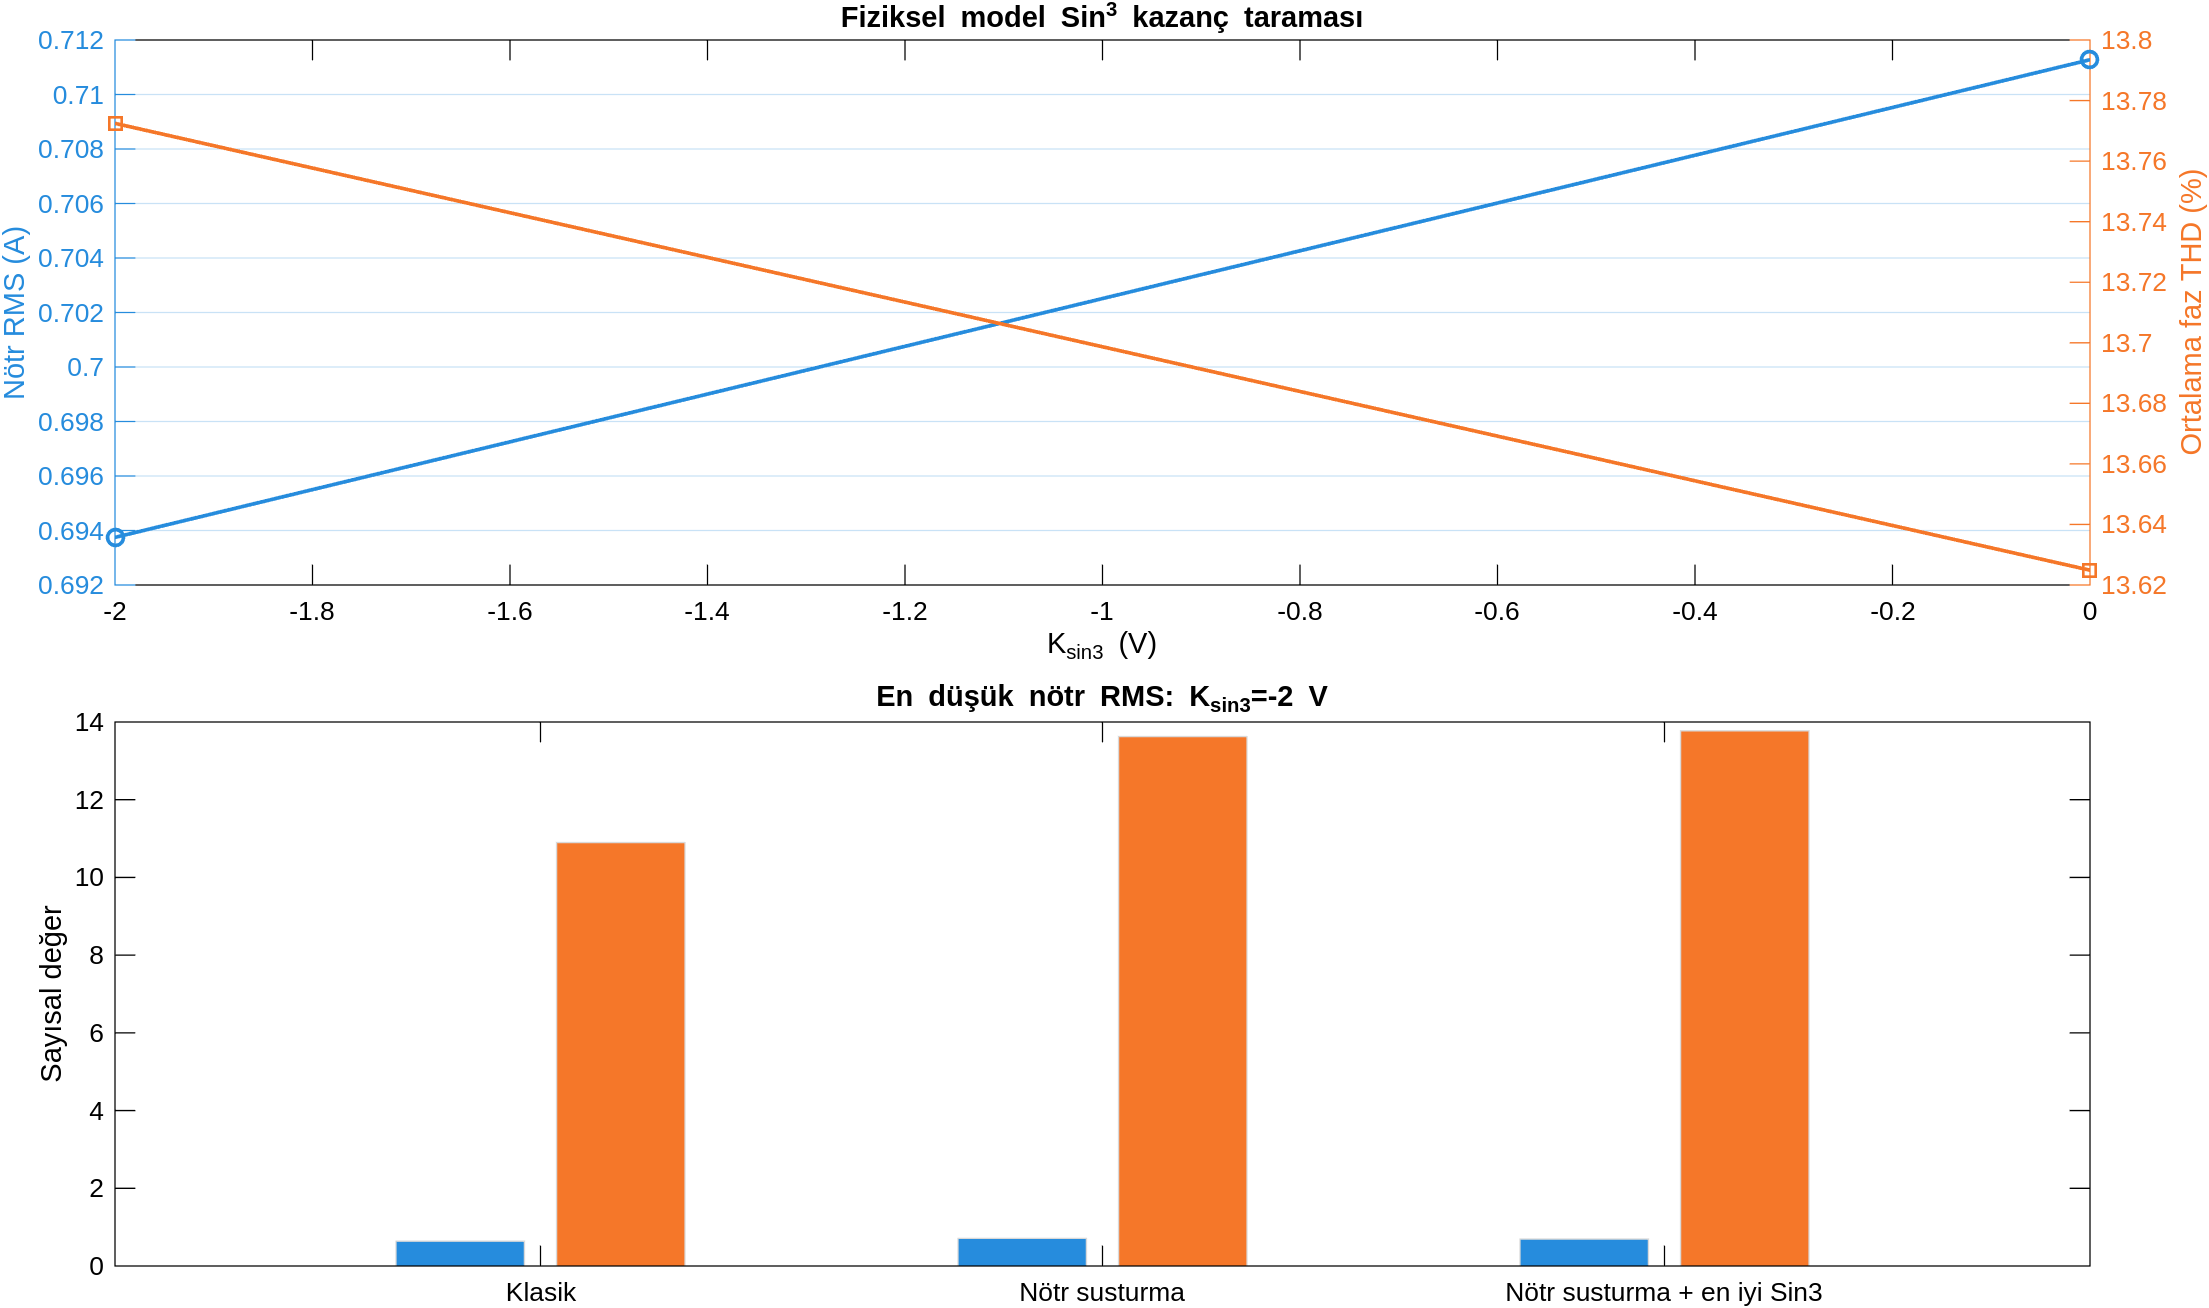
\includegraphics[width=0.96\textwidth]{sonuclar/fiziksel_senaryo123_20260822.png}
  \caption{2026-08-22 fiziksel üç faz yeniden koşusunda nötr RMS ve ortalama faz THD karşılaştırması. Sonuçlar geçici fiziksel model parametreleriyle sınırlıdır.}
  \label{fig:yeniden-uretim-fiziksel-s123}
\end{figure}

Senaryo~4 için ayrıca, gelen $L_1=\SI{600}{\micro\henry}$, $R_1=\SI{0.02}{\ohm}$, $V_{\mathrm{dc}}=\SI{431}{\volt}$ ve \SI{120}{\volt} RMS şebeke değerleriyle ortalama-değerli bir akım-döngüsü fizibilite deneyi yapılmıştır. İleri besleme $K_1\sin(\theta+\phi)+K_3\sin^3(\theta)$ biçiminde, geri besleme ise $L_1$ akımıyla çalışan PI çıkışı olarak aynı gerilim komutunda toplanmıştır. Gelen nottaki ``30~A'' ifadesi tepe mi RMS mi belirtmediğinden iki yorum da sınanmıştır. PI kazançları $K_p=\SI{3}{\volt\per\ampere}$ ve $K_i=\SI{100}{\volt\per\ampere\second}$, denetim periyodu \SI{100}{\micro\second} ve $K_3=-\SI{2}{\volt}$ seçilmiştir.

\begin{table}[htbp]
  \centering
  \caption{Senaryo~4 ortalama-değerli PI fizibilite deneyi; yarı iletken anahtarlama kaybı ve verim kapsam dışıdır.}
  \label{tab:senaryo4-pi-30a}
  \small
  \begin{tabularx}{\textwidth}{p{0.17\textwidth} X r r r r}
    \toprule
    30 A yorumu & Denetim & Ölçülen RMS (A) & RMSE (A) & THD (\%) & $|m|_{\max}$ \\
    \midrule
    Tepe (21,213 A RMS) & İleri besleme & 11,742 & 11,187 & 5,326 & 0,781 \\
    Tepe (21,213 A RMS) & İleri besleme+PI & 20,922 & 0,665 & 0,559 & 0,791 \\
    RMS & İleri besleme & 20,138 & 11,135 & 3,103 & 0,783 \\
    RMS & İleri besleme+PI & 29,715 & 0,662 & 0,393 & 0,793 \\
    \bottomrule
  \end{tabularx}
\end{table}

Her iki PI koşusunda da modülasyon doyumu oluşmamış ve referans izleme belirgin biçimde iyileşmiştir. Şekil~\ref{fig:senaryo4-pi-30a}, son iki periyottaki akımları ve modülasyon payını göstermektedir. Sonuç, yaklaşık 30~A akımın ileri besleme+PI yapısıyla ortalama modelde izlenebildiğini kanıtlar; anahtarlamalı LCL model, cihaz kayıpları, termal portlar ve gerçek PI kodu eklenmeden \%94--95 verim veya donanım kararlılığı iddiası kurmaz.

\begin{figure}[htbp]
  \centering
  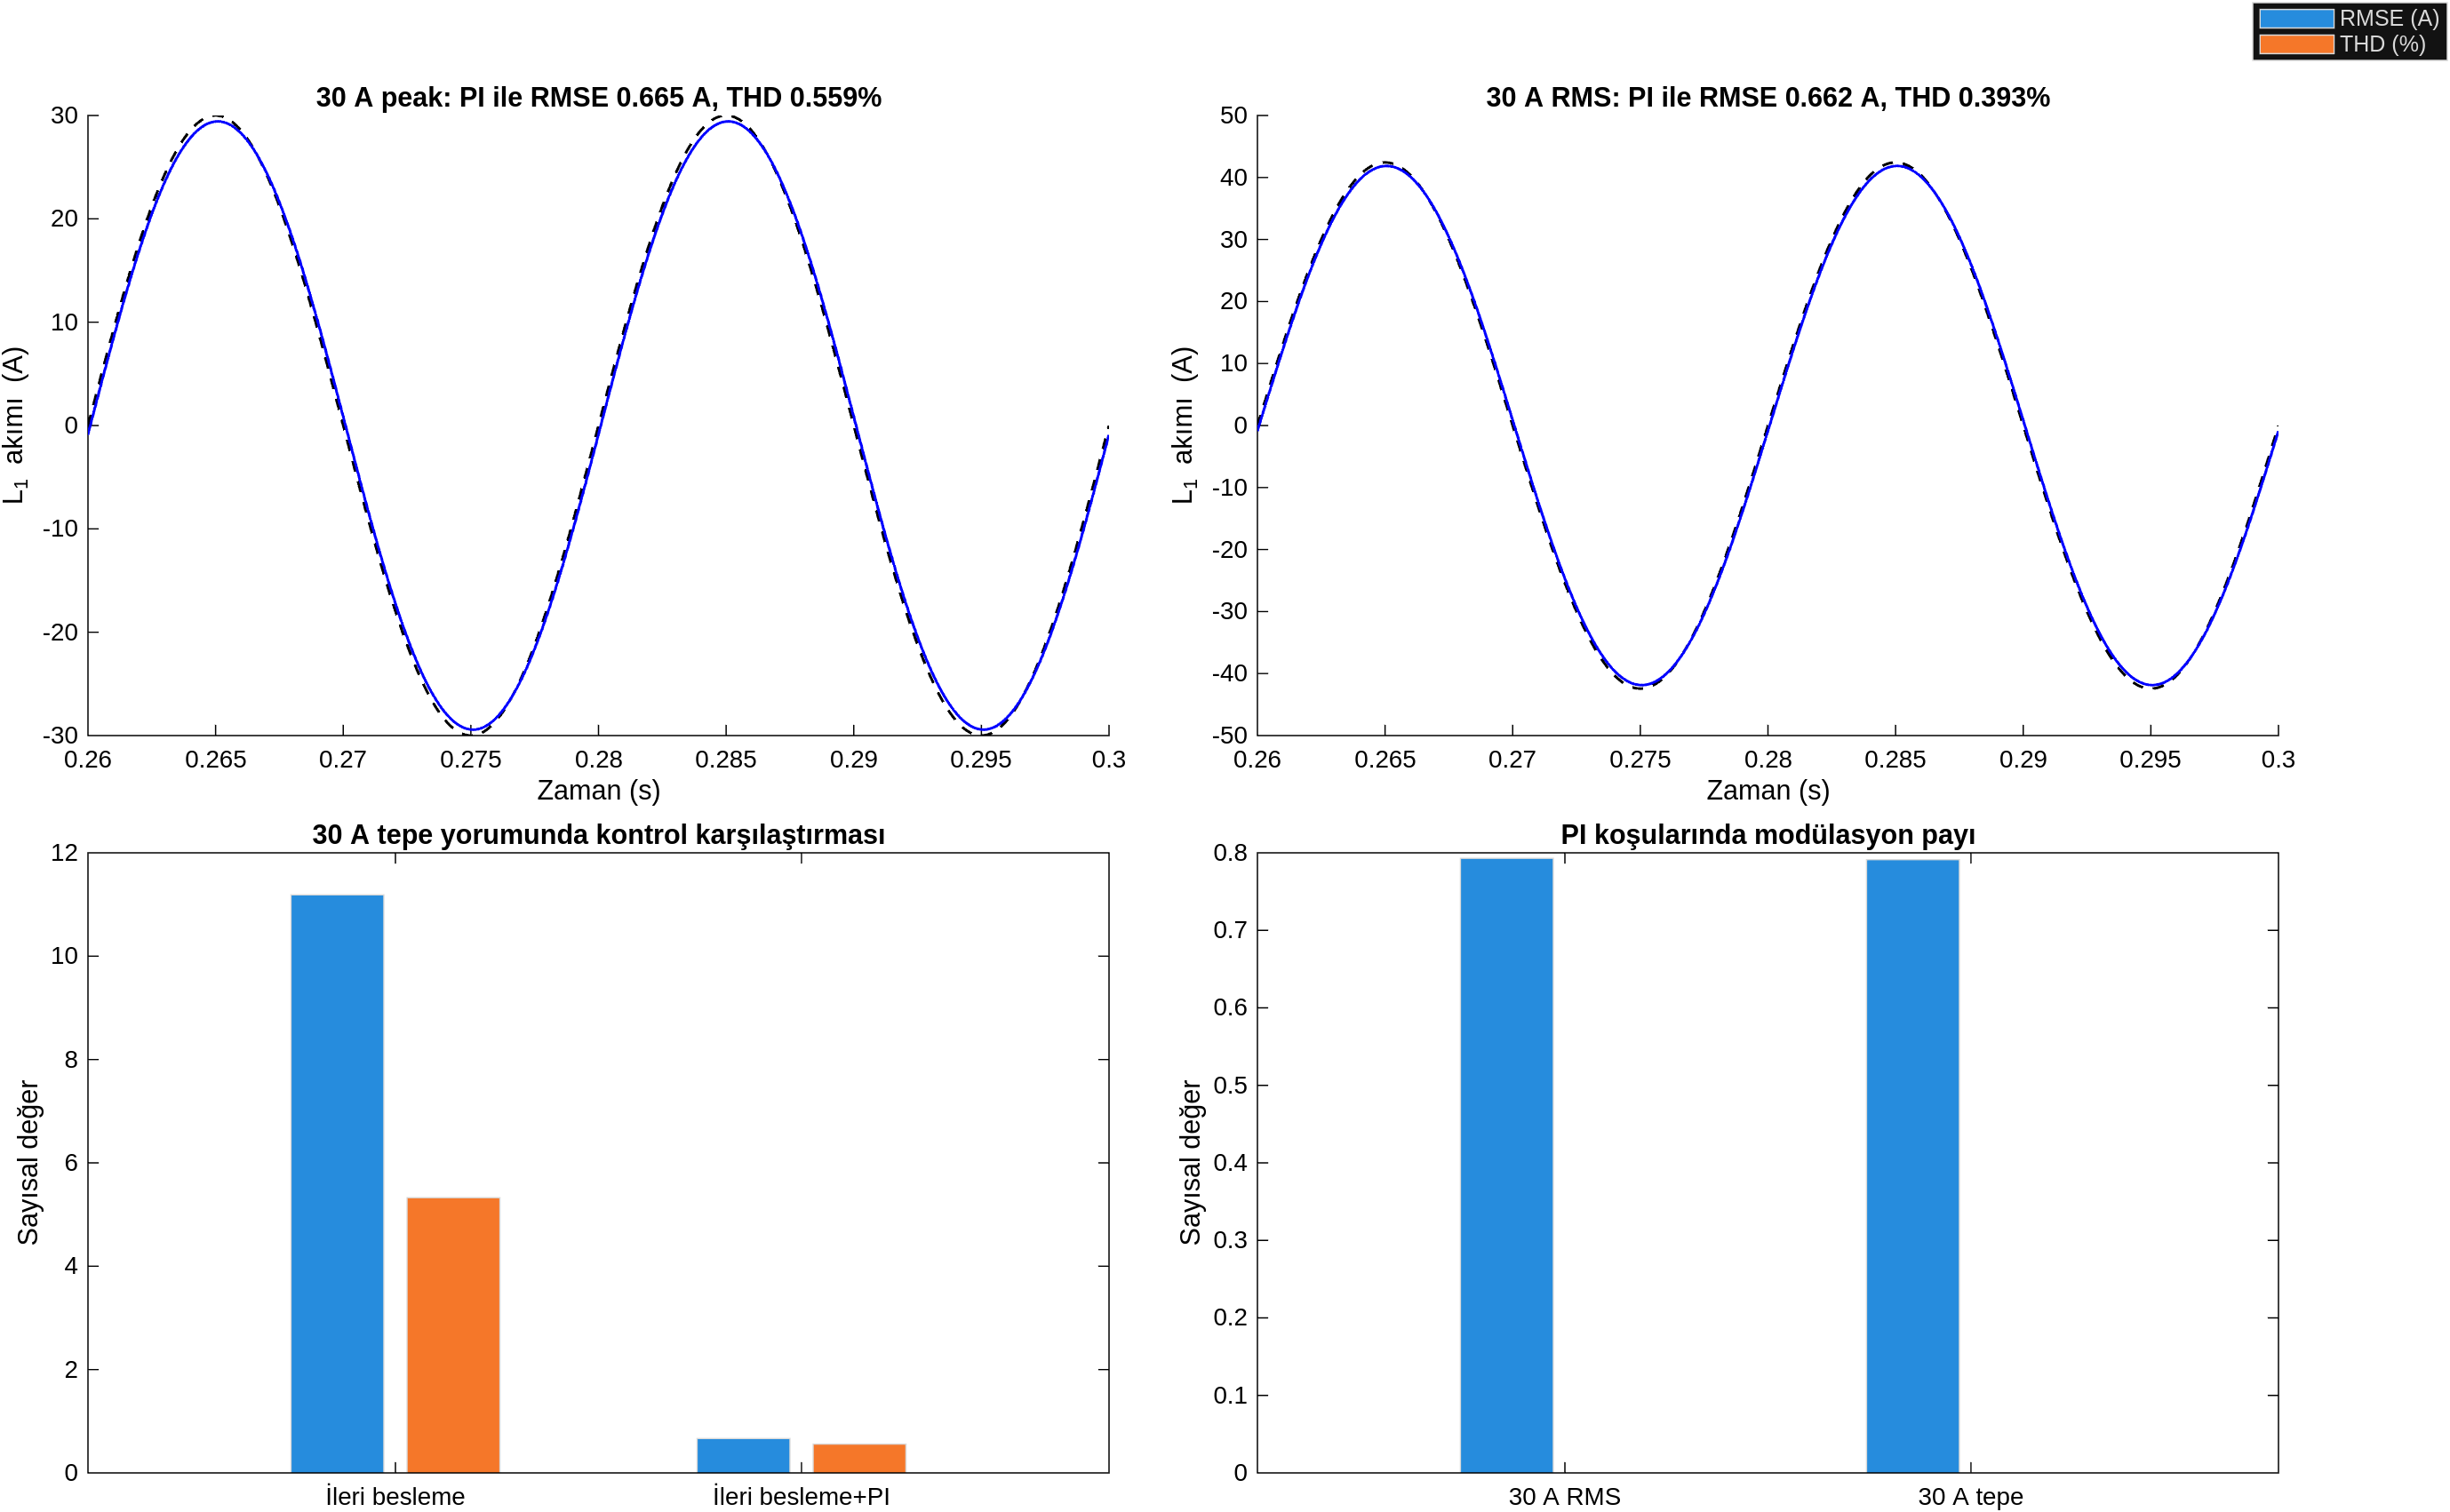
\includegraphics[width=0.98\textwidth]{sonuclar/senaryo4_pi_30a_20260822.png}
  \caption{Senaryo~4 için 30~A tepe ve 30~A RMS yorumlarında ileri besleme+PI akım izleme fizibilitesi ve modülasyon payı.}
  \label{fig:senaryo4-pi-30a}
\end{figure}

Nihai kazanç seçimi düşük güçte tek bir THD minimumuna göre yapılmayacaktır. Aday kazançlar önce düşük güçte ters akım--THD ödünleşimiyle taranacak, ardından orta ve nominal güçte kompanzasyonun gereksiz temel bileşen değişimi veya doyum üretmediği doğrulanacaktır. Aynı denetleyici katsayılarının bütün güç aralığında korunması hedeflenecek; kazanç çizelgelemesi gerekirse etkinleştirme eşiği, histerezis ve geçiş sürekliliği açıkça raporlanacaktır.

\tezcalismanotu{D5-5 --- Katkı ve üstünlük iddialarının ortak koşullu sınanması}{Sin\textsuperscript{3} kompanzasyonunun PLL/PR yapılarına göre daha basit olduğu, hesaplama yükünü veya anahtarlama sayısını azalttığı ve bütün güç aralığında THD'yi iyileştirdiği yönündeki eski tez ifadeleri henüz nihai sonuç değildir. Gerçek kodda işlem süresi/bellek, kapı başına geçiş sayısı, doyum, $I_3/I_1$, THD, RMS akım, verim ve kararlılık marjı klasik--susturma--susturma+Sin\textsuperscript{3} yöntemleri için aynı düşük, orta ve nominal güç koşullarında karşılaştırılacaktır. Yalnız desteklenen üstünlükler Bölüm~8'e taşınacaktır.}

\section{Bölüm Sonucu}

Sin\textsuperscript{3} özdeşliği temel ve üçüncü harmonik bileşenini tek bir anlık terimde birleştirmekte, ancak doğrudan $\sin(3\theta)$ enjeksiyonuyla aynı katsayı anlamını taşımamaktadır. DCM zarf modeli, nötr susturma sonrasında sinüzoidal görev oranının neden sinüzoidal akım üretmediğini göstermiştir. Eski tezin analitik taraması, katsayı yüzeyi ve Senaryo~3 ekranları korunmuş; çelişen optimumlar ile ham model eksikliği görünür biçimde sınırlandırılmıştır.

Kapalı çevrim yapı Sin\textsuperscript{3} terimini bağımsız kontrolcü olarak değil, akım döngüsünün modülasyon toplamına eklenen ileri besleme girişi olarak konumlandırmıştır. Geçici MATLAB modeli $L$, $S$ ve $T$ analiz zincirini ve şebeke endüktansı taramasını çalıştırmaktadır; sayısal kararlılık marjları gerçek parametre doğrulaması beklemektedir. 2026-08-22 fiziksel koşusu tarihsel THD iyileşmesini yeniden üretmemiş ve gerçek enjeksiyon/kazanç eşleşmesinin zorunluluğunu göstermiştir. Senaryo~4 ortalama modeli yaklaşık 30~A akımın PI ile doyumsuz izlenebildiğini göstermiştir; orta ve nominal güçte anahtarlamalı verim, termal durum, THD ve geçici rejim karşılaştırması gerçek model ve ölçüm verileriyle tamamlanmalıdır.
